\documentclass[aspectratio=169,10pt]{beamer}

\usepackage[T1]{fontenc}
\usepackage{lmodern}
\usepackage{amsmath,amssymb}
\usepackage{booktabs}
\usepackage{tabularx}
\usepackage{array}
\usepackage{graphicx}
\usepackage{listings}
\usepackage{tikz}
\usetikzlibrary{arrows.meta,calc,positioning,shapes.geometric}

% -----------------------------------------------------------------------------
% Portable 16:9 theme. No external fonts, logos, images, or theme packages are
% required. Every TikZ diagram is wrapped in \resizebox{\linewidth}{!}{...} so
% its bounding box is constrained to the current slide or column.
% -----------------------------------------------------------------------------
\definecolor{mkNavy}{HTML}{263B68}
\definecolor{mkBlue}{HTML}{246BCE}
\definecolor{mkCyan}{HTML}{1AA6A6}
\definecolor{mkGreen}{HTML}{2D8A52}
\definecolor{mkYellow}{HTML}{E0A51B}
\definecolor{mkOrange}{HTML}{D66A2C}
\definecolor{mkRed}{HTML}{B84040}
\definecolor{mkPurple}{HTML}{7557B7}
\definecolor{mkGray}{HTML}{5E6673}
\definecolor{mkLight}{HTML}{F4F7FB}
\definecolor{mkLine}{HTML}{CBD4E1}

\usetheme{Madrid}
\usecolortheme{default}
\setbeamercolor{normal text}{fg=black!88}
\setbeamercolor{structure}{fg=mkBlue}
\setbeamercolor{title}{fg=mkNavy}
\setbeamercolor{frametitle}{fg=white,bg=mkNavy}
\setbeamercolor{block title}{fg=white,bg=mkBlue}
\setbeamercolor{block body}{fg=black!88,bg=mkBlue!6}
\setbeamercolor{block title alerted}{fg=white,bg=mkOrange}
\setbeamercolor{block body alerted}{fg=black!88,bg=mkOrange!8}
\setbeamercolor{block title example}{fg=white,bg=mkGreen}
\setbeamercolor{block body example}{fg=black!88,bg=mkGreen!8}
\setbeamertemplate{navigation symbols}{}
\setbeamertemplate{footline}{%
  \leavevmode%
  \hbox{%
    \begin{beamercolorbox}[wd=.82\paperwidth,ht=2.6ex,dp=1.1ex,leftskip=1em]{author in head/foot}%
      MosaicKV Design and Implementation
    \end{beamercolorbox}%
    \begin{beamercolorbox}[wd=.18\paperwidth,ht=2.6ex,dp=1.1ex,center]{date in head/foot}%
      \insertframenumber/\inserttotalframenumber
    \end{beamercolorbox}%
  }%
}

\newcommand{\code}[1]{\texttt{\detokenize{#1}}}
\newcommand{\whylabel}{\textbf{Why do we need it?}}
\newcommand{\safetylabel}{\textbf{Safety rule:}}
\newcommand{\teachinglabel}{\textcolor{mkPurple}{\textbf{Teaching example---not a measurement}}}
\newcommand{\tightitems}{\setlength{\itemsep}{0.28em}\setlength{\parskip}{0pt}}

\lstdefinestyle{mosaickv}{
  basicstyle=\ttfamily\scriptsize,
  backgroundcolor=\color{mkLight},
  frame=single,
  rulecolor=\color{mkLine},
  breaklines=true,
  columns=fullflexible,
  keepspaces=true,
  showstringspaces=false
}

\tikzset{
  mkbox/.style={draw=mkLine,very thick,rounded corners=2pt,fill=white,
    align=center,minimum height=0.72cm,inner sep=4pt,font=\scriptsize},
  mkblue/.style={mkbox,draw=mkBlue,fill=mkBlue!7},
  mkcyan/.style={mkbox,draw=mkCyan,fill=mkCyan!8},
  mkgreen/.style={mkbox,draw=mkGreen,fill=mkGreen!9},
  mkyellow/.style={mkbox,draw=mkYellow,fill=mkYellow!13},
  mkorange/.style={mkbox,draw=mkOrange,fill=mkOrange!10},
  mkpurple/.style={mkbox,draw=mkPurple,fill=mkPurple!8},
  mkarrow/.style={-{Latex[length=2.3mm]},very thick,draw=mkGray},
  mkdasharrow/.style={-{Latex[length=2.3mm]},very thick,dashed,draw=mkPurple},
  mklabel/.style={font=\scriptsize,align=center,text=mkGray}
}

\title[MosaicKV Design]{MosaicKV (MKV): Design and Implementation}
\subtitle{A detailed, plain-language guide to multimodal key--value cache compression}
\author{MosaicKV Project}
\institute{Training-free Multimodal Inference Research}
\date{Design-document slide edition \textbullet{} 4 August 2026}

\begin{document}

% 1 ---------------------------------------------------------------------------
\begin{frame}
  \titlepage
  \vspace{-1.2em}
  \begin{center}
    \small
    Goal: understand what every component does, why it exists, how it is implemented,
    and where it is currently safe to run.
  \end{center}
\end{frame}

% 2 ---------------------------------------------------------------------------
\begin{frame}{How to Read This Deck}
\small
\begin{columns}[T,onlytextwidth]
\column{0.48\textwidth}
\begin{block}{For a new learner}
\begin{itemize}\tightitems
  \item Every technical word is expanded before its abbreviation.
  \item Each component includes a simple analogy.
  \item Figures explain the idea before equations do.
  \item Equations use only symbols defined on the slide.
\end{itemize}
\end{block}
\column{0.48\textwidth}
\begin{alertblock}{Scientific boundary}
\begin{itemize}\tightitems
  \item This is a design and implementation deck.
  \item Fictional numbers are labeled teaching examples.
  \item No small exploratory run is presented as a paper result.
  \item Unsupported paths are shown as unsupported.
\end{itemize}
\end{alertblock}
\end{columns}
\vspace{0.6em}
\begin{exampleblock}{One sentence summary}
MKV packs the most useful model memories into a smaller active cache, safely summarizes some
related memories, and can restore originals when decoding becomes risky.
\end{exampleblock}
\end{frame}

% 3 ---------------------------------------------------------------------------
\begin{frame}{Abbreviations I: Model and Runtime Keywords}
\scriptsize
\begin{tabularx}{\textwidth}{>{\bfseries}p{0.14\textwidth}p{0.31\textwidth}X}
\toprule
Short form & Full keyword & Simple meaning \\
\midrule
VLM & Vision--Language Model & A model that reasons over words and visual inputs. \\
LM & Language Model & The part that produces the answer one token at a time. \\
Q/K/V & Query / Key / Value & Search request / search label / returned information. \\
KV cache & Key--Value cache & Saved K/V tensors reused during generation. \\
FullKV & Full Key--Value reference & The untouched ground-truth cache. \\
HF & Hugging Face Transformers & The primary owned model runtime. \\
CPU/GPU & Central / Graphics Processing Unit & Host processor / accelerator. \\
RoPE & Rotary Position Embedding & A position-dependent rotation used in attention. \\
M-RoPE & Multimodal RoPE & Qwen2.5-VL's temporal, height, and width rotations. \\
GQA & Grouped-Query Attention & Several query heads share one KV head. \\
\bottomrule
\end{tabularx}
\end{frame}

% 4 ---------------------------------------------------------------------------
\begin{frame}{Abbreviations II: The Six MosaicKV Components}
\scriptsize
\begin{tabularx}{\textwidth}{>{\bfseries}p{0.14\textwidth}p{0.34\textwidth}X}
\toprule
Short form & Full keyword & Job inside MKV \\
\midrule
FQF & Future-Query Forecasting & Predict what future decode steps may search for. \\
SCEG & Sparse Cross-Modal Evidence Graph & Connect related text, image, layout, and video blocks. \\
VBU & Value-Aware Block Utility & Score future attention, value effect, novelty, and evidence. \\
BSS & Budgeted Submodular Selection & Choose useful, diverse blocks under a hard budget. \\
ET & Exact Tier & Keep selected K/V blocks unchanged. \\
PT & Prototype Tier & Keep safe summaries of compatible unselected blocks. \\
RT & Residual Tier & Store original PT members on the CPU for recovery. \\
TTC & Three-Tier Cache & ET, PT, and RT together. \\
UGRR & Uncertainty-Guided Residual Repair & Restore selected originals during risky decode steps. \\
DAR & Decision-Aware Repair & UGRR that also checks the next-token probability margin. \\
\bottomrule
\end{tabularx}
\end{frame}

% 5 ---------------------------------------------------------------------------
\begin{frame}{Abbreviations III: Safety, Evaluation, and Storage}
\scriptsize
\begin{tabularx}{\textwidth}{>{\bfseries}p{0.14\textwidth}p{0.34\textwidth}X}
\toprule
Short form & Full keyword & Simple meaning \\
\midrule
LPM & Logical Position Map & Maps packed cache slots to original token positions. \\
KVBD & KV Block Descriptor & Metadata for one selectable cache block. \\
PKT & Prototype Key Transform & Safely removes and reapplies RoPE for PT keys. \\
PAR/EPR & Prompt-Anchor / Evidence-Preservation Reservation & Budgeted safety blocks retained before greedy selection. \\
LFC/PHR & Label-Free Fidelity Calibration / Per-Head Routing & Freeze robust settings without answer-label tuning. \\
DPCB & Dense Physical Cache Budget & Budget adjusted to the memory HF truly allocates. \\
RR & Retention Ratio & Active compressed KV bytes divided by FullKV KV bytes. \\
TTFT/ITL/E2E & Time To First Token / Inter-Token Latency / End To End & Three timing boundaries. \\
KL/MSE & Kullback--Leibler divergence / Mean Squared Error & Distribution and reconstruction error. \\
\bottomrule
\end{tabularx}
\end{frame}

\begin{frame}{Abbreviations IV: Data, Numbers, and Software}
\scriptsize
\begin{tabularx}{\textwidth}{>{\bfseries}p{0.16\textwidth}p{0.35\textwidth}X}
\toprule
Short form & Full keyword & Simple meaning \\
\midrule
BL & Baseline & A comparison method used to judge MKV. \\
OCR & Optical Character Recognition & Text/layout extracted from an image. \\
COO/CSR & Coordinate / Compressed Sparse Row & Two sparse-graph storage formats. \\
FP32/FP16/BF16 & 32-bit / 16-bit / brain floating point & Numerical compute/storage formats. \\
FP8/INT8 & 8-bit floating point / integer & Smaller optional RT formats. \\
JSON/JSONL & JavaScript Object Notation / JSON Lines & Structured result and log files. \\
YAML/CLI & YAML Ain't Markup Language / Command-Line Interface & Configuration file / run command. \\
SHA & Secure Hash Algorithm identifier & Fingerprint for code, config, or profile. \\
CUDA & Compute Unified Device Architecture & NVIDIA GPU software platform. \\
NaN/Inf & Not a Number / Infinity & Invalid numerical values rejected by checks. \\
\bottomrule
\end{tabularx}
\end{frame}

% 6 ---------------------------------------------------------------------------
\begin{frame}{Roadmap}
\small
\begin{columns}[T,onlytextwidth]
\column{0.31\textwidth}
\begin{block}{Part 1: Foundations}
\begin{enumerate}\tightitems
  \item Tokens and attention
  \item Why KV cache exists
  \item Memory problem
  \item FullKV ground truth
\end{enumerate}
\end{block}
\column{0.35\textwidth}
\begin{block}{Part 2: MKV Design}
\begin{enumerate}\tightitems
  \setcounter{enumi}{4}
  \item FQF and SCEG
  \item VBU and BSS
  \item ET/PT/RT
  \item UGRR and DAR
\end{enumerate}
\end{block}
\column{0.30\textwidth}
\begin{block}{Part 3: Implementation}
\begin{enumerate}\tightitems
  \setcounter{enumi}{8}
  \item Runtime and adapters
  \item Tests and provenance
  \item Backend support
  \item Limitations
\end{enumerate}
\end{block}
\end{columns}
\end{frame}

\section{Foundations}

% 7 ---------------------------------------------------------------------------
\begin{frame}{A VLM Turns Everything into Tokens}
\small
\begin{center}
\resizebox{0.93\linewidth}{!}{%
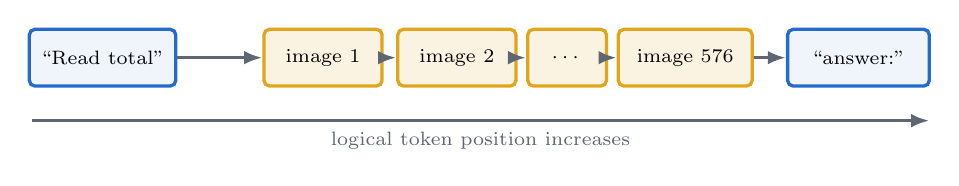
\begin{tikzpicture}[x=1cm,y=1cm]
  \node[mkblue,minimum width=1.8cm] (texta) at (0,0) {``Read total''};
  \node[mkyellow,minimum width=1.5cm] (imga) at (2.8,0) {image 1};
  \node[mkyellow,minimum width=1.5cm] (imgb) at (4.5,0) {image 2};
  \node[mkyellow,minimum width=1.0cm] (dots) at (5.9,0) {$\cdots$};
  \node[mkyellow,minimum width=1.7cm] (imgz) at (7.4,0) {image 576};
  \node[mkblue,minimum width=1.8cm] (textb) at (9.6,0) {``answer:''};
  \draw[mkarrow] (texta)--(imga);
  \draw[mkarrow] (imga)--(imgb);
  \draw[mkarrow] (imgb)--(dots);
  \draw[mkarrow] (dots)--(imgz);
  \draw[mkarrow] (imgz)--(textb);
  \draw[mkarrow] (-0.9,-0.8) -- node[below,mklabel] {logical token position increases} (10.5,-0.8);
\end{tikzpicture}}
\end{center}
\begin{columns}[T,onlytextwidth]
\column{0.47\textwidth}
\begin{block}{Text}
A tokenizer splits words into small pieces called text tokens.
\end{block}
\column{0.49\textwidth}
\begin{block}{Images and video}
A vision encoder and projector turn visual patches or frames into language-side visual tokens.
\end{block}
\end{columns}
\begin{alertblock}{\whylabel}
One image may add hundreds of tokens; documents, multiple images, and video can add much more.
\end{alertblock}
\end{frame}

% 8 ---------------------------------------------------------------------------
\begin{frame}{Attention Is a Search through Stored Notes}
\small
\begin{columns}[T,onlytextwidth]
\column{0.52\textwidth}
\resizebox{\linewidth}{!}{%
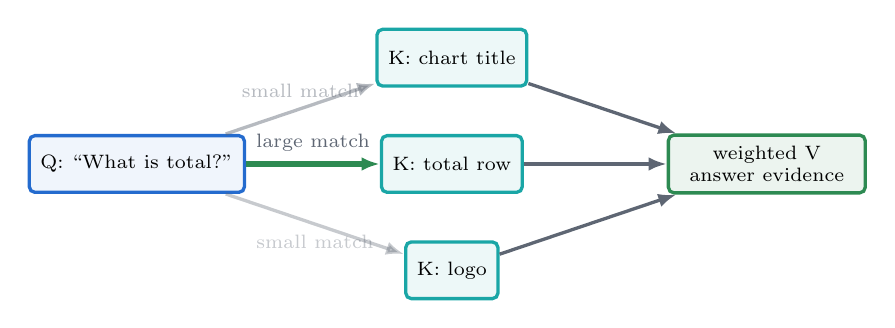
\begin{tikzpicture}[x=1cm,y=1cm]
  \node[mkblue,minimum width=2.4cm] (q) at (0,0) {Q: ``What is total?''};
  \node[mkcyan] (k1) at (4,1.35) {K: chart title};
  \node[mkcyan] (k2) at (4,0) {K: total row};
  \node[mkcyan] (k3) at (4,-1.35) {K: logo};
  \node[mkgreen,minimum width=2.5cm] (o) at (8,0) {weighted V\\answer evidence};
  \draw[mkarrow,opacity=.45] (q)--node[above,mklabel] {small match}(k1);
  \draw[-{Latex[length=2.3mm]},line width=2.2pt,draw=mkGreen] (q)--node[above,mklabel] {large match}(k2);
  \draw[mkarrow,opacity=.35] (q)--node[below,mklabel] {small match}(k3);
  \draw[mkarrow] (k1)--(o);
  \draw[mkarrow] (k2)--(o);
  \draw[mkarrow] (k3)--(o);
\end{tikzpicture}}
\column{0.44\textwidth}
\begin{block}{Three roles}
\begin{itemize}\tightitems
  \item \textbf{Q}: what the current token wants.
  \item \textbf{K}: how a stored token can be found.
  \item \textbf{V}: information returned when found.
\end{itemize}
\end{block}
\begin{exampleblock}{Notebook analogy}
Q is a question, K is an index-card label, and V is the note written on the card.
\end{exampleblock}
\end{columns}
\end{frame}

% 9 ---------------------------------------------------------------------------
\begin{frame}{The Attention Equation---One Step at a Time}
\small
\begin{columns}[T,onlytextwidth]
\column{0.55\textwidth}
\begin{align*}
  s_j &= \frac{qk_j^{\mathsf T}}{\sqrt d}
  &&\text{compare Q with each K},\\[0.25em]
  a_j &= \operatorname{softmax}(s)_j
  &&\text{turn scores into probabilities},\\[0.25em]
  o &= \sum_j a_jv_j
  &&\text{mix V using those probabilities}.
\end{align*}
\column{0.41\textwidth}
\begin{block}{Symbols}
\begin{itemize}\tightitems
  \item $j$: stored token position
  \item $d$: attention-head size
  \item $a_j$: attention probability
  \item $o$: attention output
\end{itemize}
\end{block}
\end{columns}
\begin{alertblock}{Compression danger}
If a useful K/V pair disappears, its probability or returned evidence can no longer influence $o$.
\end{alertblock}
\end{frame}

% 10 --------------------------------------------------------------------------
\begin{frame}{Why the KV Cache Exists}
\small
\begin{center}
\resizebox{0.93\linewidth}{!}{%
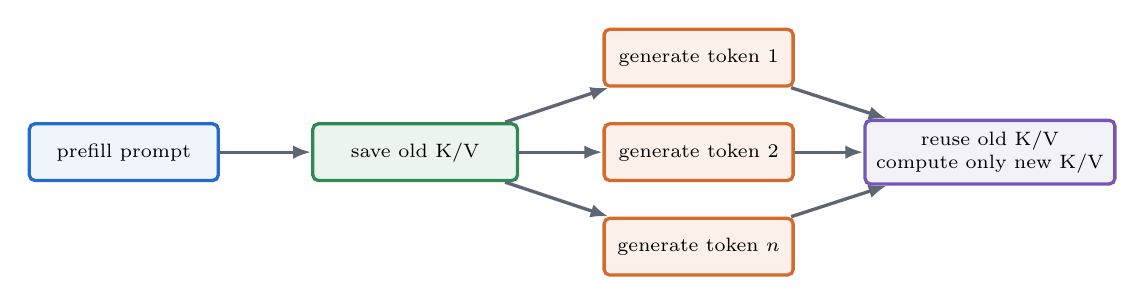
\begin{tikzpicture}[x=1cm,y=1cm]
  \node[mkblue,minimum width=2.4cm] (prefill) at (0,0) {prefill prompt};
  \node[mkgreen,minimum width=2.6cm] (cache) at (3.7,0) {save old K/V};
  \node[mkorange,minimum width=2.4cm] (t1) at (7.3,1.2) {generate token 1};
  \node[mkorange,minimum width=2.4cm] (t2) at (7.3,0) {generate token 2};
  \node[mkorange,minimum width=2.4cm] (tn) at (7.3,-1.2) {generate token $n$};
  \node[mkpurple,minimum width=2.5cm] (reuse) at (11,0) {reuse old K/V\\compute only new K/V};
  \draw[mkarrow] (prefill)--(cache);
  \draw[mkarrow] (cache)--(t1);
  \draw[mkarrow] (cache)--(t2);
  \draw[mkarrow] (cache)--(tn);
  \draw[mkarrow] (t1)--(reuse);
  \draw[mkarrow] (t2)--(reuse);
  \draw[mkarrow] (tn)--(reuse);
\end{tikzpicture}}
\end{center}
\begin{block}{Benefit}
Without a KV cache, the LM would recompute old K/V after every generated token. The cache trades
GPU memory for much less repeated computation.
\end{block}
\begin{alertblock}{New problem}
The cache is helpful, but a long multimodal prefix can consume a large share of GPU memory.
\end{alertblock}
\end{frame}

% 11 --------------------------------------------------------------------------
\begin{frame}{Why Multimodal KV Memory Grows Quickly}
\small
For a common dense cache layout $[B,H_{KV},L,D]$:
\[
\text{KV bytes}\approx
2\times N_{layers}\times B\times H_{KV}\times L\times D
\times \text{bytes per number}.
\]
\begin{columns}[T,onlytextwidth]
\column{0.47\textwidth}
\begin{block}{What grows?}
\begin{itemize}\tightitems
  \item $L$: text + image + document + video tokens
  \item $N_{layers}$: decoder depth
  \item $H_{KV}$: KV heads
  \item $B$: concurrent batch size
\end{itemize}
\end{block}
\column{0.49\textwidth}
\begin{alertblock}{Why 2?}
The cache stores both keys (K) and values (V). Every additional prompt token adds K/V data in
every decoder layer.
\end{alertblock}
\end{columns}
\end{frame}

% 12 --------------------------------------------------------------------------
\begin{frame}{Research Problem}
\large
\begin{center}
\begin{minipage}{0.90\textwidth}
\begin{block}{The challenge}
After one full multimodal prefill, keep enough task-relevant evidence for accurate deterministic
decoding while obeying a hard active-KV byte budget---without training or changing model weights.
\end{block}
\end{minipage}
\end{center}
\vspace{0.5em}
\small
\begin{columns}[T,onlytextwidth]
\column{0.31\textwidth}
\begin{exampleblock}{Quality}
Keep evidence needed by future answer tokens.
\end{exampleblock}
\column{0.31\textwidth}
\begin{exampleblock}{Systems}
Reduce actual active GPU KV bytes under a fixed budget.
\end{exampleblock}
\column{0.31\textwidth}
\begin{exampleblock}{Correctness}
Preserve positions, cache meaning, and deterministic behavior.
\end{exampleblock}
\end{columns}
\end{frame}

% 13 --------------------------------------------------------------------------
\begin{frame}{FullKV Is the Ground Truth}
\small
\begin{columns}[T,onlytextwidth]
\column{0.47\textwidth}
\begin{block}{FullKV does}
\begin{itemize}\tightitems
  \item one ordinary full-cache prefill;
  \item deterministic greedy decoding;
  \item synchronized timing and memory measurement.
\end{itemize}
\end{block}
\column{0.49\textwidth}
\begin{alertblock}{FullKV never does}
\begin{itemize}\tightitems
  \item pruning or prototype merging;
  \item quantization or offloading;
  \item residual storage or repair.
\end{itemize}
\end{alertblock}
\end{columns}
\vspace{0.5em}
\begin{exampleblock}{Identity gate at RR = 1.0}
Every MKV source block must remain exact. PT and RT must be empty. Token output and compared logits
must reproduce FullKV within the preregistered numerical tolerance.
\end{exampleblock}
\end{frame}

% 14 --------------------------------------------------------------------------
\begin{frame}{Why Simple Top-$k$ Pruning Is Not Enough}
\small
\begin{tabularx}{\textwidth}{>{\bfseries}p{0.26\textwidth}X}
\toprule
Simple decision & Possible failure \\
\midrule
Keep highest prompt attention & Future answer queries may need different evidence. \\
Score each token alone & Many selected tokens may repeat the same fact. \\
Ignore modality/layout & A chart cell can lose its row/column label. \\
Average any nearby K/V & Post-RoPE keys can have incompatible phases. \\
Compress once forever & A surprising future token cannot correct a bad decision. \\
Compare nominal token ratios & Methods may use different actual bytes. \\
\bottomrule
\end{tabularx}
\begin{alertblock}{MKV design response}
Forecast future need, connect shared evidence, reward diversity, merge only safely, preserve
recoverable originals, and repair only when uncertainty justifies it.
\end{alertblock}
\end{frame}

\section{MosaicKV Overview}

% 15 --------------------------------------------------------------------------
\begin{frame}{The Six-Part MosaicKV Design}
\small
\begin{center}
\resizebox{0.98\linewidth}{!}{%
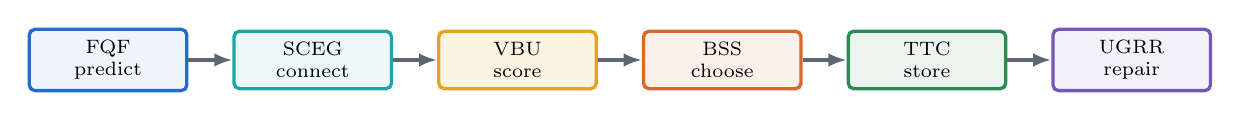
\begin{tikzpicture}[x=1cm,y=1cm]
  \node[mkblue,minimum width=2.0cm] (f) at (0,0) {FQF\\predict};
  \node[mkcyan,minimum width=2.0cm] (g) at (2.6,0) {SCEG\\connect};
  \node[mkyellow,minimum width=2.0cm] (u) at (5.2,0) {VBU\\score};
  \node[mkorange,minimum width=2.0cm] (s) at (7.8,0) {BSS\\choose};
  \node[mkgreen,minimum width=2.0cm] (t) at (10.4,0) {TTC\\store};
  \node[mkpurple,minimum width=2.0cm] (r) at (13.0,0) {UGRR\\repair};
  \draw[mkarrow] (f)--(g);
  \draw[mkarrow] (g)--(u);
  \draw[mkarrow] (u)--(s);
  \draw[mkarrow] (s)--(t);
  \draw[mkarrow] (t)--(r);
\end{tikzpicture}}
\end{center}
\begin{block}{Why the order matters}
Each stage supplies information or safety to the next: future need $\rightarrow$ evidence links
$\rightarrow$ utility $\rightarrow$ diverse selection $\rightarrow$ representation
$\rightarrow$ correction.
\end{block}
\begin{alertblock}{System contract}
Removing a component creates a named ablation. It must not be silently renamed ``MosaicKV full.''
\end{alertblock}
\end{frame}

% 16 --------------------------------------------------------------------------
\begin{frame}{End-to-End Runtime}
\scriptsize
\begin{center}
\resizebox{0.98\linewidth}{!}{%
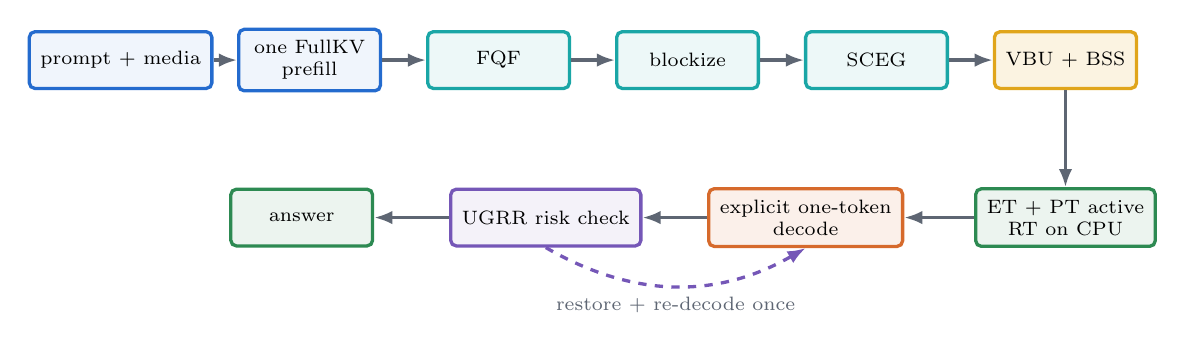
\begin{tikzpicture}[x=1cm,y=1cm]
  \node[mkblue,minimum width=1.8cm] (in) at (0,1.2) {prompt + media};
  \node[mkblue,minimum width=1.8cm] (pf) at (2.4,1.2) {one FullKV\\prefill};
  \node[mkcyan,minimum width=1.8cm] (fq) at (4.8,1.2) {FQF};
  \node[mkcyan,minimum width=1.8cm] (bl) at (7.2,1.2) {blockize};
  \node[mkcyan,minimum width=1.8cm] (gr) at (9.6,1.2) {SCEG};
  \node[mkyellow,minimum width=1.8cm] (se) at (12.0,1.2) {VBU + BSS};
  \node[mkgreen,minimum width=2.0cm] (tier) at (12.0,-0.8) {ET + PT active\\RT on CPU};
  \node[mkorange,minimum width=2.0cm] (decode) at (8.7,-0.8) {explicit one-token\\decode};
  \node[mkpurple,minimum width=2.0cm] (risk) at (5.4,-0.8) {UGRR risk check};
  \node[mkgreen,minimum width=1.8cm] (out) at (2.3,-0.8) {answer};
  \draw[mkarrow] (in)--(pf); \draw[mkarrow] (pf)--(fq); \draw[mkarrow] (fq)--(bl);
  \draw[mkarrow] (bl)--(gr); \draw[mkarrow] (gr)--(se); \draw[mkarrow] (se)--(tier);
  \draw[mkarrow] (tier)--(decode); \draw[mkarrow] (decode)--(risk); \draw[mkarrow] (risk)--(out);
  \draw[mkdasharrow] (risk.south) to[bend right=30] node[below,mklabel] {restore + re-decode once} (decode.south);
\end{tikzpicture}}
\end{center}
\begin{block}{One owned path}
FullKV, BL methods, and MKV share message preparation, decoding, byte accounting, measurement,
result writing, and failure recording.
\end{block}
\end{frame}

% 17 --------------------------------------------------------------------------
\begin{frame}{The Explicit HF Runtime Owns the Cache}
\small
\begin{columns}[T,onlytextwidth]
\column{0.51\textwidth}
\begin{block}{Why not use \code{model.generate()}?}
MKV must inspect and modify the cache between prefill and decoding. A hidden generation loop does
not expose a safe transaction boundary for this work.
\end{block}
\begin{block}{Owned operations}
\begin{itemize}\tightitems
  \item prepare inputs;
  \item prefill once;
  \item extract/inject model-specific cache;
  \item decode exactly one token;
  \item capture Q vectors and eager attention.
\end{itemize}
\end{block}
\column{0.45\textwidth}
\begin{alertblock}{Determinism}
\begin{itemize}\tightitems
  \item temperature $=0$;
  \item sampling disabled;
  \item greedy \code{argmax};
  \item same terminal tokens;
  \item same maximum output length.
\end{itemize}
\end{alertblock}
\end{columns}
\end{frame}
% 18 --------------------------------------------------------------------------
\begin{frame}{Model Adapter Contract}
\scriptsize
\begin{tabularx}{\textwidth}{>{\bfseries}p{0.31\textwidth}X}
\toprule
Adapter operation & Purpose \\
\midrule
\code{prepare_inputs} & Apply the exact chat template and media processor. \\
\code{prefill} & Run one full prompt pass and expose cache, logits, Q, and optional attention. \\
\code{decode_one_token} & Advance one deterministic token with explicit state. \\
\code{extract_past_key_values} & Snapshot the actual model-specific cache class and layout. \\
\code{inject_past_key_values} & Rebuild a compatible cache after compression or repair. \\
\code{capture_query_vectors} & Hook every decoder \code{q_proj} without changing weights. \\
\code{get_modality_map} & Mark text, image, and video spans. \\
\code{get_cache_layout} & Record shapes, dtypes, devices, sequence axes, and key RoPE state. \\
\code{build_prototype_key_transform} & Supply an audited PKT or declare PT unsupported. \\
\bottomrule
\end{tabularx}
\begin{alertblock}{\whylabel}
Different VLM families use different processors, cache classes, and position rules. The adapter
keeps those model-specific facts out of generic MKV algorithms.
\end{alertblock}
\end{frame}

\section{Cache State and Blocks}

% 19 --------------------------------------------------------------------------
\begin{frame}{Logical Position Is Not Physical Storage Position}
\small
\begin{center}
\resizebox{0.89\linewidth}{!}{%
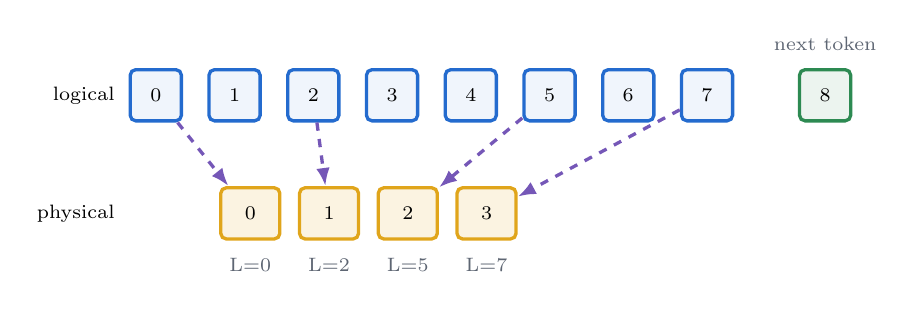
\begin{tikzpicture}[x=1cm,y=1cm]
  \node[anchor=east,font=\scriptsize] at (-0.4,1.4) {logical};
  \foreach \x in {0,...,7}{\node[mkblue,minimum width=.65cm,minimum height=.65cm,inner sep=1pt] (l\x) at (\x,1.4) {\x};}
  \node[mkgreen,minimum width=.65cm,minimum height=.65cm,inner sep=1pt] (next) at (8.5,1.4) {8};
  \node[above=1mm of next,mklabel] {next token};
  \node[anchor=east,font=\scriptsize] at (-0.4,-0.1) {physical};
  \foreach \x/\logical in {0/0,1/2,2/5,3/7}{
    \node[mkyellow,minimum width=.75cm,minimum height=.65cm,inner sep=1pt] (p\x) at (\x+1.2,-0.1) {\x};
    \node[below=1mm of p\x,mklabel] {L=\logical};
  }
  \draw[mkdasharrow] (l0)--(p0); \draw[mkdasharrow] (l2)--(p1);
  \draw[mkdasharrow] (l5)--(p2); \draw[mkdasharrow] (l7)--(p3);
\end{tikzpicture}}
\end{center}
\begin{block}{Three separate values}
Original logical length $=8$; packed active length $=4$; next decode position $=8$.
\end{block}
\begin{alertblock}{\safetylabel}
Do not renumber positions after pruning. RoPE and causal decoding use original logical positions.
\end{alertblock}
\end{frame}

% 20 --------------------------------------------------------------------------
\begin{frame}{The Logical Position Map (LPM)}
\small
\begin{columns}[T,onlytextwidth]
\column{0.48\textwidth}
\begin{block}{LPM stores}
\begin{itemize}\tightitems
  \item physical-to-logical position mapping;
  \item original prompt sequence length;
  \item next decode position;
  \item active packed length.
\end{itemize}
\end{block}
\column{0.48\textwidth}
\begin{exampleblock}{Backpack analogy}
Moving pages into a smaller binder changes their binder slots, not their original page numbers.
The table of contents must still point to the original numbers.
\end{exampleblock}
\end{columns}
\vspace{0.55em}
\begin{alertblock}{Implementation invariant}
Logical positions are strictly increasing inside each block, and every generated token advances
from the original prompt length rather than the packed length.
\end{alertblock}
\end{frame}

% 21 --------------------------------------------------------------------------
\begin{frame}{Fixed-Size Blockization}
\small
\begin{center}
\resizebox{0.96\linewidth}{!}{%
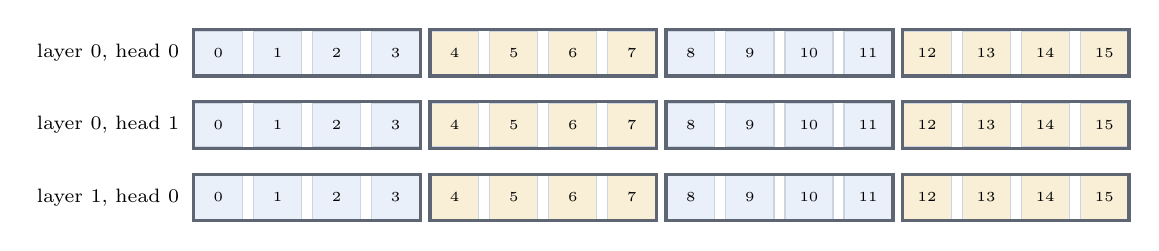
\begin{tikzpicture}[x=.75cm,y=.8cm]
  \foreach \row/\label in {0/{layer 0, head 0},1/{layer 0, head 1},2/{layer 1, head 0}}{
    \node[anchor=east,font=\scriptsize] at (-.5,{2.2-1.15*\row}) {\label};
    \foreach \x in {0,...,15}{
      \pgfmathtruncatemacro{\group}{int(\x/4)}
      \pgfmathtruncatemacro{\shade}{mod(\group,2)}
      \ifnum\shade=0\def\tone{mkBlue!10}\else\def\tone{mkYellow!18}\fi
      \node[draw=mkLine,fill=\tone,minimum width=.61cm,minimum height=.55cm,inner sep=0pt,font=\tiny]
        at (\x,{2.2-1.15*\row}) {\x};
    }
    \foreach \x in {0,4,8,12}{
      \draw[very thick,draw=mkGray] (\x-.42,{2.57-1.15*\row}) rectangle (\x+3.42,{1.83-1.15*\row});
    }
  }
\end{tikzpicture}}
\end{center}
\begin{block}{Example block size $b=4$}
Four consecutive cache positions form a selectable unit. Blockization repeats independently for
every layer and KV head.
\end{block}
\begin{alertblock}{\safetylabel}
Never combine different layers or KV heads in one block. Split at required modality/metadata
boundaries, and never remove a mandatory block.
\end{alertblock}
\end{frame}

% 22 --------------------------------------------------------------------------
\begin{frame}{What a KV Block Descriptor (KVBD) Records}
\scriptsize
\begin{columns}[T,onlytextwidth]
\column{0.48\textwidth}
\begin{block}{Cache identity}
\begin{itemize}\tightitems
  \item layer and KV head;
  \item physical cache indices;
  \item original logical positions;
  \item token IDs, when available;
  \item K/V dtype and device;
  \item exact payload byte size.
\end{itemize}
\end{block}
\column{0.48\textwidth}
\begin{block}{Evidence identity}
\begin{itemize}\tightitems
  \item text, image, or video modality;
  \item image, frame, page, and region IDs;
  \item normalized image box;
  \item OCR, row, column, and page-region metadata;
  \item mandatory/non-compressible flag.
\end{itemize}
\end{block}
\end{columns}
\begin{alertblock}{\whylabel}
Selection needs both tensor cost and evidence meaning. KVBD makes every decision and byte auditable.
\end{alertblock}
\end{frame}

% 23 --------------------------------------------------------------------------
\begin{frame}{Block-State Invariants}
\small
\begin{enumerate}\tightitems
  \item Every source position belongs to exactly one source block in its layer/head.
  \item ET membership never conflicts with PT or RT source ownership.
  \item PT and RT overlap only through the declared recovery relationship.
  \item Active-byte accounting equals the underlying ET/PT tensor storage.
  \item At RR $=1.0$, exact reinjection reconstructs the original cache.
  \item Mandatory blocks always remain exact.
  \item Logical positions remain monotonic inside every block.
\end{enumerate}
\begin{exampleblock}{Why check these during construction?}
A late failure during decode is difficult to diagnose. Typed state objects reject contradictory
ownership, invalid positions, and incorrect bytes before generation begins.
\end{exampleblock}
\end{frame}

\section{Future-Query Forecasting}

% 24 --------------------------------------------------------------------------
\begin{frame}{Component 1: Future-Query Forecasting (FQF)}
\small
\begin{columns}[T,onlytextwidth]
\column{0.50\textwidth}
\begin{block}{Question FQF asks}
``What kinds of evidence will the model probably search for while it writes the answer?''
\end{block}
\begin{exampleblock}{Simple analogy}
Before cleaning a desk, imagine the next homework questions. Keep notes likely to be useful, not
only notes used by the previous question.
\end{exampleblock}
\column{0.46\textwidth}
\begin{alertblock}{Why prompt attention alone can fail}
\begin{itemize}\tightitems
  \item The prompt reads the input.
  \item The answer may compare, calculate, or format.
  \item Those future actions can produce different Q vectors and attention.
\end{itemize}
\end{alertblock}
\end{columns}
\end{frame}

% 25 --------------------------------------------------------------------------
\begin{frame}{Three FQF Modes}
\scriptsize
\begin{tabularx}{\textwidth}{>{\bfseries}p{0.19\textwidth}p{0.34\textwidth}X}
\toprule
Mode & What it uses & Why use it? \\
\midrule
Prompt Window (PW) & Q and attention from the final $w$ prompt positions. & Cheapest; the end of
the question often describes the answer type. \\
Draft Rollout (DR) & $r$ temporary FullKV greedy decode steps. & Closer to real future answer
queries, but costs extra decode time. \\
Hybrid Query Forecast (HQF) & PW statistics plus DR samples. & Keeps a prompt safety anchor while
following heads that shift during drafting. \\
\bottomrule
\end{tabularx}
\vspace{0.5em}
\begin{alertblock}{Valid zero settings}
PW requires $w>0,r=0$; DR requires $w=0,r>0$; HQF requires both $w>0$ and $r>0$.
\end{alertblock}
\end{frame}

% 26 --------------------------------------------------------------------------
\begin{frame}{Draft Rollout Reuses One Prefill}
\small
\begin{center}
\resizebox{0.95\linewidth}{!}{%
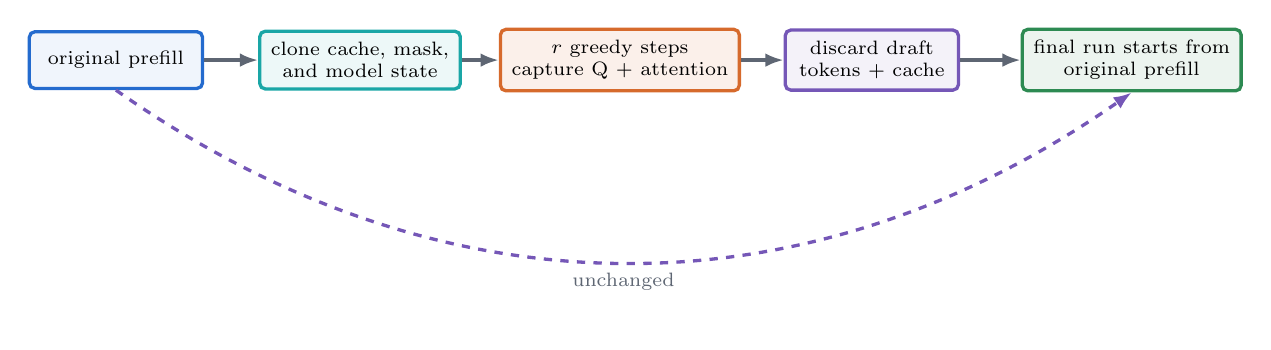
\begin{tikzpicture}[x=1cm,y=1cm]
  \node[mkblue,minimum width=2.2cm] (pf) at (0,0) {original prefill};
  \node[mkcyan,minimum width=2.2cm] (clone) at (3.1,0) {clone cache, mask,\\and model state};
  \node[mkorange,minimum width=2.3cm] (draft) at (6.4,0) {$r$ greedy steps\\capture Q + attention};
  \node[mkpurple,minimum width=2.2cm] (discard) at (9.6,0) {discard draft\\tokens + cache};
  \node[mkgreen,minimum width=2.4cm] (final) at (12.9,0) {final run starts from\\original prefill};
  \draw[mkarrow] (pf)--(clone); \draw[mkarrow] (clone)--(draft);
  \draw[mkarrow] (draft)--(discard); \draw[mkarrow] (discard)--(final);
  \draw[mkdasharrow] (pf.south) to[bend right=35] node[below,mklabel] {unchanged} (final.south);
\end{tikzpicture}}
\end{center}
\begin{block}{Two critical rules}
No second prefill is allowed. The draft state must not share mutable K/V tensors with the final
state; an integrity check compares the original state before and after drafting.
\end{block}
\end{frame}

% 27 --------------------------------------------------------------------------
\begin{frame}{What the Query Forecast (QF) Stores}
\scriptsize
For every decoder layer and KV head, \code{QueryForecast} stores:
\begin{columns}[T,onlytextwidth]
\column{0.47\textwidth}
\begin{block}{Statistics}
\begin{itemize}\tightitems
  \item PW mean $\mu$;
  \item full covariance $\Sigma$ or diagonal variance;
  \item DR query samples;
  \item normalized centroids $c_1,\dots,c_K$;
  \item centroid weights $\pi_1,\dots,\pi_K$.
\end{itemize}
\end{block}
\column{0.49\textwidth}
\begin{block}{Provenance and cost}
\begin{itemize}\tightitems
  \item layer, KV head, and contributing Q heads;
  \item exact PW positions and sample counts;
  \item mode, covariance type, and centroid method;
  \item cache-isolation checks;
  \item separate clone, draft, statistics, and centroid timing.
\end{itemize}
\end{block}
\end{columns}
\begin{alertblock}{Low-memory option}
Streaming spherical centroids use $O(KD)$ extra centroid memory rather than a full sample-by-centroid
assignment matrix.
\end{alertblock}
\end{frame}

% 28 --------------------------------------------------------------------------
\begin{frame}{GQA and Per-Head Forecast Routing}
\small
\begin{columns}[T,onlytextwidth]
\column{0.49\textwidth}
\begin{block}{Grouped-Query Attention (GQA)}
When several Q heads share one KV head, all those Q heads become forecast samples for that KV head.
The runtime rejects a Q-head count that is not divisible by the KV-head count.
\end{block}
\column{0.47\textwidth}
\begin{block}{Adaptive routing}
Compare PW and DR attention distributions per KV head. Stable heads can favor PW; shifted heads can
receive more DR weight.
\end{block}
\end{columns}
\begin{alertblock}{\whylabel}
One global prompt/draft mixture assumes every head changes in the same way. Per-head routing keeps
stable evidence while allowing changed heads to follow future behavior.
\end{alertblock}
\end{frame}

% 29 --------------------------------------------------------------------------
\begin{frame}{Important RoPE Boundary in FQF}
\small
\begin{center}
\resizebox{0.84\linewidth}{!}{%
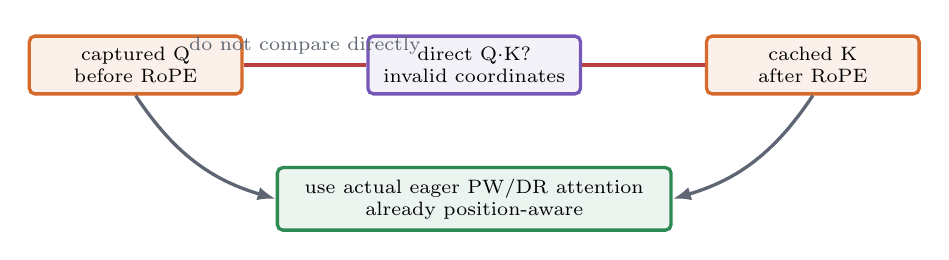
\begin{tikzpicture}[x=1cm,y=1cm]
  \node[mkorange,minimum width=2.7cm] (q) at (0,0) {captured Q\\before RoPE};
  \node[mkpurple,minimum width=2.7cm] (bad) at (4.3,0) {direct Q$\cdot$K?\\invalid coordinates};
  \node[mkorange,minimum width=2.7cm] (k) at (8.6,0) {cached K\\after RoPE};
  \draw[-,very thick,draw=mkRed] (q)--node[above,mklabel] {do not compare directly}(bad);
  \draw[-,very thick,draw=mkRed] (bad)--(k);
  \node[mkgreen,minimum width=5.0cm] (good) at (4.3,-1.7) {use actual eager PW/DR attention\\already position-aware};
  \draw[mkarrow] (q.south) to[bend right=20] (good.west);
  \draw[mkarrow] (k.south) to[bend left=20] (good.east);
\end{tikzpicture}}
\end{center}
\begin{alertblock}{\safetylabel}
VBU accepts only explicitly RoPE-aware attention provenance. Pre-RoPE Q is never silently dotted
with post-RoPE K and called valid attention.
\end{alertblock}
\end{frame}

% 30 --------------------------------------------------------------------------
\begin{frame}{How FQF Quality Is Diagnosed}
\small
\begin{itemize}\tightitems
  \item \textbf{Q cosine similarity}: does a centroid point toward true future Q?
  \item \textbf{Attention rank correlation}: are blocks ordered similarly to true future attention?
  \item \textbf{Selected-block recall}: how many oracle-selected blocks did FQF help retain?
  \item \textbf{Forecast regret}: how much true future attention mass was missed?
\end{itemize}
\begin{alertblock}{Evaluation-only oracle}
True future Q and attention come from a cloned FullKV decode in a separate evaluation namespace.
They may measure FQF, but can never enter online compression decisions.
\end{alertblock}
\begin{exampleblock}{Why internal diagnostics matter}
A final answer may be correct by luck. These metrics test whether FQF actually predicted useful
future evidence.
\end{exampleblock}
\end{frame}

\section{Evidence Graph and Selection}

% 31 --------------------------------------------------------------------------
\begin{frame}{Component 2: Sparse Cross-Modal Evidence Graph (SCEG)}
\small
\begin{columns}[T,onlytextwidth]
\column{0.49\textwidth}
\begin{block}{Question SCEG asks}
``Which cache blocks may be different pieces of the same evidence?''
\end{block}
\begin{exampleblock}{Simple analogy}
Draw strings between a chart legend, its colored bar, its axis label, and the words in the question.
The strings show that the notes belong together.
\end{exampleblock}
\column{0.47\textwidth}
\begin{alertblock}{Why token order is not enough}
\begin{itemize}\tightitems
  \item A row header and numeric cell can be far apart.
  \item A question word and image region use different modalities.
  \item Related video evidence may occur in nearby frames.
\end{itemize}
\end{alertblock}
\end{columns}
\end{frame}

% 32 --------------------------------------------------------------------------
\begin{frame}{A Small SCEG Example}
\small
\begin{center}
\resizebox{0.80\linewidth}{!}{%
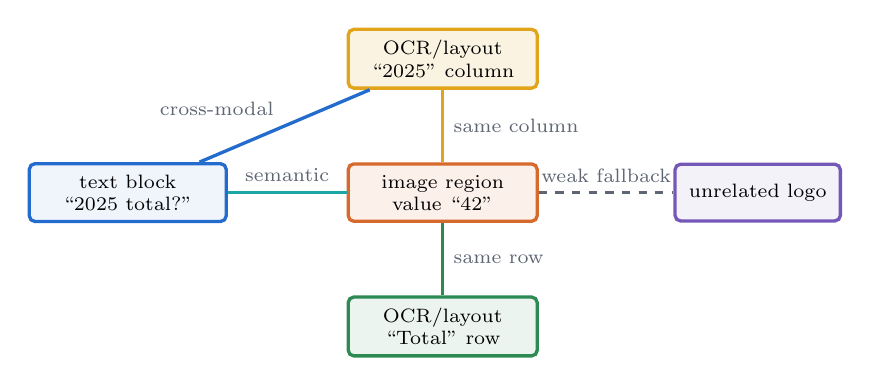
\begin{tikzpicture}[x=1cm,y=1cm]
  \node[mkblue,minimum width=2.5cm] (q) at (0,0) {text block\\``2025 total?''};
  \node[mkyellow,minimum width=2.4cm] (col) at (4,1.7) {OCR/layout\\``2025'' column};
  \node[mkorange,minimum width=2.4cm] (cell) at (4,0) {image region\\value ``42''};
  \node[mkgreen,minimum width=2.4cm] (row) at (4,-1.7) {OCR/layout\\``Total'' row};
  \node[mkpurple,minimum width=2.1cm] (logo) at (8,0) {unrelated logo};
  \draw[-,very thick,draw=mkBlue] (q)--node[above left,mklabel] {cross-modal}(col);
  \draw[-,very thick,draw=mkCyan] (q)--node[above,mklabel] {semantic}(cell);
  \draw[-,very thick,draw=mkYellow] (col)--node[right,mklabel] {same column}(cell);
  \draw[-,very thick,draw=mkGreen] (row)--node[right,mklabel] {same row}(cell);
  \draw[-,thick,dashed,draw=mkGray] (cell)--node[above,mklabel] {weak fallback}(logo);
\end{tikzpicture}}
\end{center}
\teachinglabel
\begin{block}{Graph meaning}
Nodes are KV blocks. Typed, weighted edges represent evidence relationships; they do not change
the actual cache tensors.
\end{block}
\end{frame}

% 33 --------------------------------------------------------------------------
\begin{frame}{SCEG Edge Types}
\scriptsize
\begin{tabularx}{\textwidth}{>{\bfseries}p{0.24\textwidth}p{0.42\textwidth}X}
\toprule
Edge & What connects? & Why useful? \\
\midrule
Semantic similarity & Similar pooled descriptors & Same meaning at distant positions \\
Attention co-activation & Blocks viewed together by PW queries & Model-observed prompt relation \\
Spatial adjacency & Nearby normalized image boxes & Charts, diagrams, nearby objects \\
OCR/layout & Same OCR text, row, column, reading order, or page region & Documents and tables \\
Temporal adjacency & Nearby frame or clip indices & Local video events \\
Same evidence region & Shared region identifier & Pieces of one detected fact \\
Cross-modal alignment & Related blocks from different modalities & Question text to visual answer \\
Fallback & Nearby compatible blocks when metadata is absent & Usable without invented metadata \\
\bottomrule
\end{tabularx}
\end{frame}

% 34 --------------------------------------------------------------------------
\begin{frame}{SCEG Compatibility Filters Prevent Invalid Links}
\small
Before adding an edge, the implementation checks:
\begin{enumerate}\tightitems
  \item same decoder layer, unless explicitly disabled for an ablation;
  \item same KV head, unless explicitly disabled;
  \item an allowed directed modality pair, such as \code{text:image};
  \item maximum logical-position span where the edge source requires locality;
  \item real spatial, OCR, page, or frame metadata when that edge type requires it.
\end{enumerate}
\begin{alertblock}{\safetylabel}
Missing metadata does not create imaginary OCR boxes, page regions, or frame identities. It uses
a labeled fallback graph instead.
\end{alertblock}
\end{frame}

% 35 --------------------------------------------------------------------------
\begin{frame}{How the SCEG Stays Sparse}
\small
\begin{columns}[T,onlytextwidth]
\column{0.52\textwidth}
\begin{block}{Avoid the $n^2$ graph}
\begin{itemize}\tightitems
  \item retain top $d$ neighbors per node and edge source;
  \item compute similarity in bounded chunks;
  \item use spatial grid buckets;
  \item use bounded layout/temporal neighborhoods;
  \item store Coordinate (COO) or Compressed Sparse Row (CSR) arrays.
\end{itemize}
\end{block}
\column{0.44\textwidth}
\begin{exampleblock}{Memory shape}
With fixed neighbor count $d$:
\[
\text{stored graph memory}=O(nd).
\]
The normal path never stores a full $n\times n$ matrix.
\end{exampleblock}
\end{columns}
\begin{alertblock}{\whylabel}
A cache-compression method must not replace saved KV memory with a giant dense graph.
\end{alertblock}
\end{frame}

% 36 --------------------------------------------------------------------------
\begin{frame}{SCEG Diagnostics}
\small
Each debug trace records:
\begin{itemize}\tightitems
  \item number of nodes and typed edges;
  \item average degree and connected components;
  \item modality mixing and edge-source counts;
  \item evidence-cluster and selected-set coverage;
  \item whether structural metadata or a fallback was used.
\end{itemize}
\begin{exampleblock}{What can diagnostics reveal?}
An empty graph can mean missing metadata or overly strict filters. A nearly dense graph can mean
bad thresholds. No cross-modal edges can reveal a modality-map problem.
\end{exampleblock}
\end{frame}

% 37 --------------------------------------------------------------------------
\begin{frame}{Component 3: Value-Aware Block Utility (VBU)}
\scriptsize
For each block $i$, VBU records seven separate signals:
\begin{enumerate}\tightitems
  \item future attention probability $p_i$;
  \item value novelty $n_i$ relative to SCEG neighbors;
  \item expected attention-output contribution $c_i$;
  \item SCEG centrality and singleton coverage;
  \item modality rarity;
  \item redundancy, the complement of novelty;
  \item mandatory priority.
\end{enumerate}
\begin{alertblock}{\whylabel}
Attention says ``will this block be viewed?'' Value contribution asks ``could it change the
output?'' Novelty asks ``is another selected block already saying the same thing?''
\end{alertblock}
\end{frame}

% 38 --------------------------------------------------------------------------
\begin{frame}{VBU Local Utility Equation}
\small
\[
u_i=\lambda_qp_i-\lambda_vc_i-\lambda_on_i.
\]
\begin{columns}[T,onlytextwidth]
\column{0.51\textwidth}
\begin{block}{Default signed coefficients}
\[
\lambda_q=1,\qquad \lambda_v=-0.25,\qquad \lambda_o=-0.25.
\]
The explicit minus signs plus negative value/novelty coefficients make those two terms rewards.
\end{block}
\column{0.45\textwidth}
\begin{alertblock}{Why signs matter}
Assuming every $\lambda$ is positive would make the equation appear to punish important, unique
evidence. The resolved signed values are always recorded.
\end{alertblock}
\end{columns}
\begin{exampleblock}{Normalization}
$p_i$, $c_i$, and $n_i$ each use a nonnegative unit-sum scale inside every layer/KV-head stratum.
\end{exampleblock}
\end{frame}

% 39 --------------------------------------------------------------------------
\begin{frame}{Prompt and Evidence Safety Reservations}
\small
\begin{columns}[T,onlytextwidth]
\column{0.48\textwidth}
\begin{block}{Prompt-Anchor Reservation (PAR)}
Keep a configured budget fraction of the strongest prompt-only attention blocks before ordinary
greedy selection.
\end{block}
\column{0.48\textwidth}
\begin{block}{Evidence-Preservation Reservation (EPR)}
Keep a configured budget fraction of blocks with strong fine-grained SCEG evidence scores.
\end{block}
\end{columns}
\begin{alertblock}{\whylabel}
PAR protects against a bad future forecast. EPR protects chart/document structure that a broad
semantic representative may blur.
\end{alertblock}
\begin{exampleblock}{Fair budget rule}
PAR and EPR consume the same active-byte budget; they are not free extra memory. Their selection
reasons are recorded separately.
\end{exampleblock}
\end{frame}

% 40 --------------------------------------------------------------------------
\begin{frame}{Component 4: Budgeted Submodular Selection (BSS)}
\small
\[
F(S)=\sum_{i\in S}u_i-\lambda_gC_{FL}(S)-\lambda_mC_{mod}(S).
\]
\begin{itemize}\tightitems
  \item $S$: selected block set.
  \item $C_{FL}$: facility-location coverage---how well selected representatives cover SCEG nodes.
  \item $C_{mod}$: fraction of available modalities represented in $S$.
  \item Defaults $\lambda_g=\lambda_m=-0.25$ turn both coverage terms into rewards.
\end{itemize}
\begin{exampleblock}{Simple meaning of ``submodular''}
The first block covering a fact helps a lot; another nearly identical block helps less. This is
the diminishing-returns idea.
\end{exampleblock}
\end{frame}

% 41 --------------------------------------------------------------------------
\begin{frame}{Deterministic Lazy-Greedy BSS}
\scriptsize
\begin{center}
\resizebox{0.96\linewidth}{!}{%
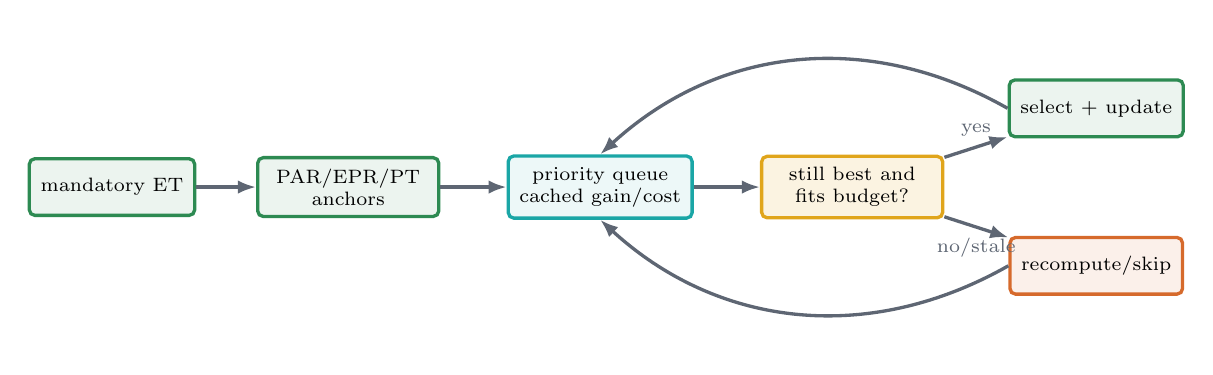
\begin{tikzpicture}[x=1cm,y=1cm]
  \node[mkgreen,minimum width=2.1cm] (m) at (0,0) {mandatory ET};
  \node[mkgreen,minimum width=2.3cm] (r) at (3.0,0) {PAR/EPR/PT\\anchors};
  \node[mkcyan,minimum width=2.3cm] (h) at (6.2,0) {priority queue\\cached gain/cost};
  \node[mkyellow,minimum width=2.3cm] (c) at (9.4,0) {still best and\\fits budget?};
  \node[mkgreen,minimum width=2.0cm] (s) at (12.5,1.0) {select + update};
  \node[mkorange,minimum width=2.0cm] (x) at (12.5,-1.0) {recompute/skip};
  \draw[mkarrow] (m)--(r); \draw[mkarrow] (r)--(h); \draw[mkarrow] (h)--(c);
  \draw[mkarrow] (c)--node[above,mklabel] {yes}(s);
  \draw[mkarrow] (c)--node[below,mklabel] {no/stale}(x);
  \draw[mkarrow] (s.west) to[bend right=36] (h.north);
  \draw[mkarrow] (x.west) to[bend left=36] (h.south);
\end{tikzpicture}}
\end{center}
\begin{block}{Tie-breaking}
Larger gain per cost, larger raw gain, lower cost, then lower node ID. Every selected and rejected
block receives a decision record.
\end{block}
\end{frame}

% 42 --------------------------------------------------------------------------
\begin{frame}{Budgets, Retention Ratio, and Exact Checks}
\small
\begin{columns}[T,onlytextwidth]
\column{0.49\textwidth}
\begin{block}{Budget units}
\begin{itemize}\tightitems
  \item blocks: cost one per block;
  \item retained slots: cost source positions;
  \item bytes: exact K/V payload bytes.
\end{itemize}
\end{block}
\column{0.47\textwidth}
\begin{block}{Realized RR}
\[
\rho_{real}=\frac{\text{measured ET + PT bytes}}
{\text{measured FullKV bytes}}.
\]
Whole blocks and dense layouts can make realized RR differ from the request.
\end{block}
\end{columns}
\begin{alertblock}{Hard rules}
Mandatory blocks are selected first. If they exceed the budget, fail. For tiny graphs, enumerate
all feasible sets and compare lazy greedy with the exact optimum.
\end{alertblock}
\end{frame}

\section{Three-Tier Cache and Repair}

% 43 --------------------------------------------------------------------------
\begin{frame}{Component 5: Three-Tier Cache (TTC)}
\small
\begin{center}
\resizebox{0.78\linewidth}{!}{%
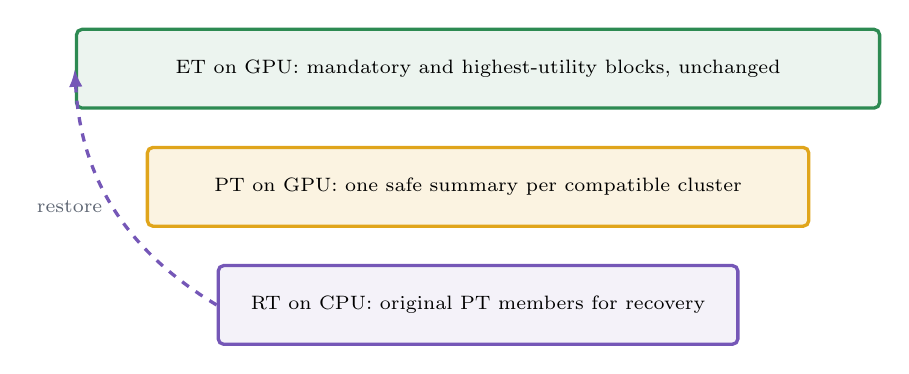
\begin{tikzpicture}[x=1cm,y=1cm]
  \node[mkgreen,minimum width=10.2cm,minimum height=1.0cm] (et) at (0,1.5)
    {ET on GPU: mandatory and highest-utility blocks, unchanged};
  \node[mkyellow,minimum width=8.4cm,minimum height=1.0cm] (pt) at (0,0)
    {PT on GPU: one safe summary per compatible cluster};
  \node[mkpurple,minimum width=6.6cm,minimum height=1.0cm] (rt) at (0,-1.5)
    {RT on CPU: original PT members for recovery};
  \draw[mkdasharrow] (rt.west) to[bend left=28] node[left,mklabel] {restore} (et.west);
\end{tikzpicture}}
\end{center}
\begin{block}{Accounting boundary}
ET + PT are active GPU KV bytes. RT is CPU residual memory and is reported separately, never hidden
inside the active budget.
\end{block}
\end{frame}

% 44 --------------------------------------------------------------------------
\begin{frame}{Exact Tier (ET): The Safety Anchor}
\small
\begin{columns}[T,onlytextwidth]
\column{0.50\textwidth}
\begin{block}{ET keeps}
\begin{itemize}\tightitems
  \item original K and V numbers;
  \item dtype and device;
  \item logical positions;
  \item layer/head identity;
  \item mandatory metadata.
\end{itemize}
\end{block}
\column{0.46\textwidth}
\begin{exampleblock}{Why exact?}
The most important evidence should not pay approximation error. ET also provides stable anchors
for PT clusters and causal generation.
\end{exampleblock}
\end{columns}
\begin{alertblock}{RR = 1.0 identity}
All source blocks go to ET; PT and RT remain empty; exact reinjection reconstructs FullKV exactly.
\end{alertblock}
\end{frame}

% 45 --------------------------------------------------------------------------
\begin{frame}{Prototype Tier (PT): Assign to Compatible Anchors}
\small
An unselected block can join an ET anchor only when it passes all rules:
\begin{enumerate}\tightitems
  \item same decoder layer;
  \item same KV head;
  \item allowed source-to-anchor modality pair;
  \item logical-position span within the configured maximum;
  \item key/value error and group-size guards, when enabled.
\end{enumerate}
\begin{block}{Anchor choice}
Prefer the highest-weight real SCEG relation. A weak bounded positional scaffold can make
representation feasible, but it is not reported as real evidence.
\end{block}
\begin{alertblock}{Fail closed}
If any unselected block lacks a safe anchor or the resulting ET + PT exceeds budget, use an
explicit exact-only fallback or stop. Never claim partial PT coverage as a complete TTC.
\end{alertblock}
\end{frame}

% 46 --------------------------------------------------------------------------
\begin{frame}{How a Weighted Prototype Is Computed}
\small
For PT members $j=1,\dots,m$ with positive weights $w_j$:
\[
\alpha_j=\frac{w_j}{\sum_rw_r},\qquad
\bar{k}=\sum_j\alpha_j\operatorname{pool}(k_j),\qquad
\bar{v}=\sum_j\alpha_j\operatorname{pool}(v_j).
\]
\begin{columns}[T,onlytextwidth]
\column{0.49\textwidth}
\begin{block}{Numerical rule}
Pool and average in FP32, then cast the result back to the cache dtype and device.
\end{block}
\column{0.47\textwidth}
\begin{block}{Storage rule}
One prototype uses one active cache slot. Its selected anchor remains exact and is not averaged
into the PT member mean.
\end{block}
\end{columns}
\begin{alertblock}{\whylabel}
A PT keeps some information from compatible omissions instead of deleting all of it.
\end{alertblock}
\end{frame}

% 47 --------------------------------------------------------------------------
\begin{frame}{Why Directly Averaging Post-RoPE Keys Is Unsafe}
\small
\begin{center}
\resizebox{0.78\linewidth}{!}{%
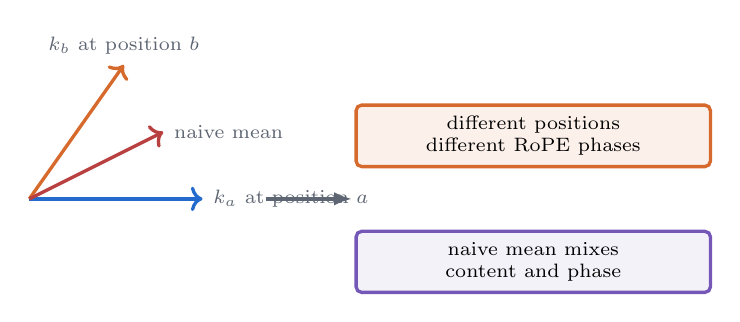
\begin{tikzpicture}[x=1cm,y=1cm]
  \draw[->,very thick,draw=mkBlue] (0,0)--(2.2,0) node[right,mklabel] {$k_a$ at position $a$};
  \draw[->,very thick,draw=mkOrange] (0,0)--(1.2,1.7) node[above,mklabel] {$k_b$ at position $b$};
  \draw[->,very thick,draw=mkRed] (0,0)--(1.7,.85) node[right,mklabel] {naive mean};
  \node[mkorange,minimum width=4.5cm] at (6.4,.8) {different positions\\different RoPE phases};
  \node[mkpurple,minimum width=4.5cm] at (6.4,-.8) {naive mean mixes\\content and phase};
  \draw[mkarrow] (3,0)--(4.1,0);
\end{tikzpicture}}
\end{center}
\begin{exampleblock}{Paper-arrow analogy}
Imagine drawing two arrows, rotating each sheet differently, and then averaging the visible
arrows. The result mixes the arrow content with the sheet rotations.
\end{exampleblock}
\end{frame}

% 48 --------------------------------------------------------------------------
\begin{frame}{Prototype Key Transform (PKT): RoPE-Safe Merging}
\scriptsize
\begin{center}
\resizebox{0.96\linewidth}{!}{%
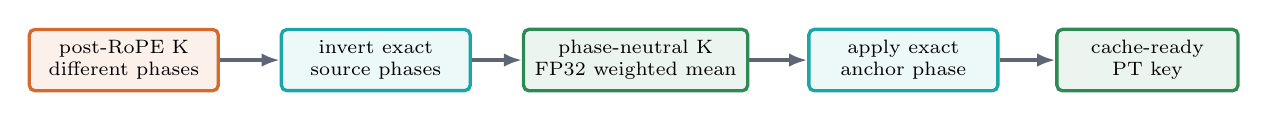
\begin{tikzpicture}[x=1cm,y=1cm]
  \node[mkorange,minimum width=2.4cm] (post) at (0,0) {post-RoPE K\\different phases};
  \node[mkcyan,minimum width=2.4cm] (inv) at (3.2,0) {invert exact\\source phases};
  \node[mkgreen,minimum width=2.6cm] (mean) at (6.5,0) {phase-neutral K\\FP32 weighted mean};
  \node[mkcyan,minimum width=2.4cm] (apply) at (9.9,0) {apply exact\\anchor phase};
  \node[mkgreen,minimum width=2.3cm] (ready) at (13.0,0) {cache-ready\\PT key};
  \draw[mkarrow] (post)--(inv); \draw[mkarrow] (inv)--(mean);
  \draw[mkarrow] (mean)--(apply); \draw[mkarrow] (apply)--(ready);
\end{tikzpicture}}
\end{center}
\begin{block}{Model-specific transforms}
Qwen2.5-VL uses exact temporal/height/width M-RoPE phases. LLaVA-1.5 and OneVision use their exact
standard Llama/Qwen2 RoPE phases for the audited request layout.
\end{block}
\begin{alertblock}{\safetylabel}
The PKT is architecture-, version-, and position-layout-specific. A mismatch disables PT rather
than averaging incompatible phases.
\end{alertblock}
\end{frame}

% 49 --------------------------------------------------------------------------
\begin{frame}{Adaptive PT and Per-Head Routing (PHR)}
\small
Not every KV head tolerates the same approximation. Label-free calibration can route a sensitive
layer/head to:
\begin{itemize}\tightitems
  \item ET only;
  \item a smaller PT group size;
  \item a shorter logical-position span;
  \item stricter key/value member-error limits.
\end{itemize}
\begin{block}{Prototype diagnostics used}
K/V dispersion, per-member reconstruction error, position span, cluster size, modality
composition, and active bytes saved.
\end{block}
\begin{alertblock}{\whylabel}
A global cluster size assumes all heads are equally robust. PHR spends exact memory where PT is
most damaging and compresses more strongly where it is safer.
\end{alertblock}
\end{frame}

% 50 --------------------------------------------------------------------------
\begin{frame}{Residual Tier (RT): Recoverable Originals}
\small
\begin{columns}[T,onlytextwidth]
\column{0.52\textwidth}
\begin{block}{RT stores}
\begin{itemize}\tightitems
  \item original unselected PT-member K/V;
  \item layer, KV head, PT ID, and positions;
  \item source dtype/device and byte offsets;
  \item contiguous CPU storage for efficient transfer.
\end{itemize}
\end{block}
\column{0.44\textwidth}
\begin{block}{Storage formats}
Lossless is the first/default path. Controlled experiments may use FP16, BF16, FP8, or symmetric
INT8 with stored scales.
\end{block}
\end{columns}
\begin{alertblock}{Pinned memory rule}
Production UGRR requires pinned CPU storage for asynchronous transfer. If requested pinning is
unavailable, fail rather than claim repair support.
\end{alertblock}
\end{frame}

% 51 --------------------------------------------------------------------------
\begin{frame}{Component 6: UGRR Signals}
\scriptsize
For provisional vocabulary probabilities $p$:
\[
H_{norm}=-\frac{\sum_xp_x\log p_x}{\log|\mathcal V|}.
\]
For PT cluster $j$:
\[
R_j=A_jD_j,
\]
where $A_j$ is globally normalized current PT attention mass and $D_j$ is K/V dispersion.
\begin{columns}[T,onlytextwidth]
\column{0.48\textwidth}
\begin{block}{Also record}
Top-two token probability margin and optional KL from a cheap draft distribution.
\end{block}
\column{0.48\textwidth}
\begin{alertblock}{Why multiple signals?}
Entropy can be high without PT being responsible. PT risk can be high while the token decision is
still confident. DAR combines relevance and decision sensitivity.
\end{alertblock}
\end{columns}
\end{frame}

% 52 --------------------------------------------------------------------------
\begin{frame}{UGRR Policies}
\scriptsize
\begin{tabularx}{\textwidth}{>{\bfseries}p{0.29\textwidth}X}
\toprule
Policy & Trigger rule \\
\midrule
none & Never repair; required control. \\
entropy & $H_{norm}$ reaches its threshold. \\
prototype risk & $\max_jR_j$ reaches its threshold and any minimum-entropy guard. \\
entropy or prototype risk & Either previous online condition is true. \\
decision aware & Very high normalized risk, or moderate risk plus a small token margin. \\
oracle & Evaluation-only counterfactual using FullKV; forbidden online. \\
\bottomrule
\end{tabularx}
\begin{alertblock}{Named behavior}
A run label records the actual policy. Oracle and online UGRR results must never be mixed.
\end{alertblock}
\end{frame}

% 53 --------------------------------------------------------------------------
\begin{frame}{A Repair Event Is a Bounded Transaction}
\scriptsize
\begin{center}
\resizebox{0.96\linewidth}{!}{%
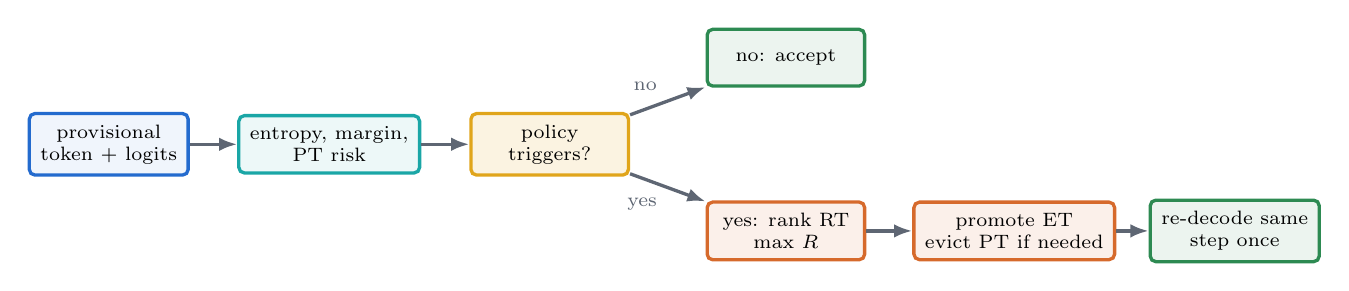
\begin{tikzpicture}[x=1cm,y=1cm]
  \node[mkblue,minimum width=2.0cm] (p) at (0,0) {provisional\\token + logits};
  \node[mkcyan,minimum width=2.0cm] (sig) at (2.8,0) {entropy, margin,\\PT risk};
  \node[mkyellow,minimum width=2.0cm] (tr) at (5.6,0) {policy\\triggers?};
  \node[mkgreen,minimum width=2.0cm] (no) at (8.6,1.1) {no: accept};
  \node[mkorange,minimum width=2.0cm] (rank) at (8.6,-1.1) {yes: rank RT\\max $R$};
  \node[mkorange,minimum width=2.0cm] (promote) at (11.5,-1.1) {promote ET\\evict PT if needed};
  \node[mkgreen,minimum width=2.0cm] (redo) at (14.3,-1.1) {re-decode same\\step once};
  \draw[mkarrow] (p)--(sig); \draw[mkarrow] (sig)--(tr);
  \draw[mkarrow] (tr)--node[above left,mklabel] {no}(no);
  \draw[mkarrow] (tr)--node[below left,mklabel] {yes}(rank);
  \draw[mkarrow] (rank)--(promote); \draw[mkarrow] (promote)--(redo);
\end{tikzpicture}}
\end{center}
\begin{alertblock}{Hard bounds}
At most $R$ originals; plan budget before transfer; re-decode count at most one; promoted blocks
remain exact for later steps.
\end{alertblock}
\end{frame}

% 54 --------------------------------------------------------------------------
\begin{frame}{Partial PT Refresh and Budget Enforcement}
\small
\begin{columns}[T,onlytextwidth]
\column{0.50\textwidth}
\begin{block}{Partial restoration}
If only some PT members are promoted, subtract them from the FP32 weighted mean, renormalize the
remaining members, and refresh dispersion. Do not discard unpromoted evidence.
\end{block}
\column{0.46\textwidth}
\begin{block}{Budget repair}
If promotion would exceed the active budget, evict the lowest-utility non-protected PT. If no
feasible plan exists, perform no transfer and record budget infeasibility.
\end{block}
\end{columns}
\begin{alertblock}{Post-RoPE rule}
For post-RoPE K, partial refresh happens in phase-neutral space through the same audited PKT.
\end{alertblock}
\end{frame}

% 55 --------------------------------------------------------------------------
\begin{frame}{Decision-Aware Repair (DAR) Calibration}
\small
\begin{enumerate}\tightitems
  \item On disjoint calibration examples, record normalized PT risk, token margin, and whether a
        FullKV counterfactual repair would have been beneficial.
  \item Search moderate-risk, high-risk, and margin thresholds.
  \item Enforce a registered maximum trigger rate and minimum predicted precision.
  \item Freeze the profile and its calibration/evaluation ledgers before held-out use.
\end{enumerate}
\begin{alertblock}{Fail-closed outcome}
If no threshold set passes the gates, the frozen profile disables online repair and predicts zero
triggers. Uncalibrated repair is not automatically enabled.
\end{alertblock}
\begin{exampleblock}{\whylabel}
A repair can change a correct token incorrectly or cost more than it helps. Calibration must show
that triggers are selective enough before DAR is trusted.
\end{exampleblock}
\end{frame}

\section{Methods, Baselines, and Worked Example}

% 56 --------------------------------------------------------------------------
\begin{frame}{Three Public MKV Methods}
\scriptsize
\begin{tabularx}{\textwidth}{>{\bfseries}p{0.22\textwidth}c c c X}
\toprule
Method & ET & PT & RT/UGRR & Meaning \\
\midrule
\code{mosaickv_exact} & yes & no & no & FQF + SCEG + VBU + BSS whole-block selection. \\
\code{mosaickv_proto} & yes & if safe & no & Exact selection plus audited PT summaries. \\
\code{mosaickv_full} & yes & if safe & if safe & Complete ET/PT/RT path with configured UGRR. \\
\bottomrule
\end{tabularx}
\vspace{0.55em}
\begin{alertblock}{Effective method label}
An unsafe PT path records an exact-only safety-fallback label. A fallback row is not PT evidence,
and a zero-trigger or unsupported repair path is not described as repaired MKV.
\end{alertblock}
\end{frame}

% 57 --------------------------------------------------------------------------
\begin{frame}{Baseline (BL) Landscape}
\scriptsize
\begin{tabularx}{\textwidth}{>{\bfseries}p{0.25\textwidth}p{0.34\textwidth}X}
\toprule
BL & Main decision & Missing relative to full MKV \\
\midrule
FullKV & Keep all K/V. & No compression. \\
Random KV & Random exact blocks with recorded seed. & No evidence signal. \\
Prompt Attention Top-$k$ & PW attention only. & No DR, value, graph coverage, PT, or UGRR. \\
\code{lookm_reimpl} & LOOK-M text prior, pivots, and own merge. & Different scoring/merge; not official code. \\
\code{prefixkv_reimpl} & Offline layer-wise prefix budgets. & No request-specific SCEG/VBU. \\
\code{vl_cache_reimpl} & VL-Cache modality sparsity and layer allocation. & Paper-derived policy, not MKV TTC; no official code assumed. \\
\bottomrule
\end{tabularx}
\begin{alertblock}{Naming rule}
Local paper-faithful implementations end in \code{_reimpl} and are never called official code.
\end{alertblock}
\end{frame}

% 58 --------------------------------------------------------------------------
\begin{frame}{What Is Structurally Different about MKV?}
\small
\begin{center}
\resizebox{0.93\linewidth}{!}{%
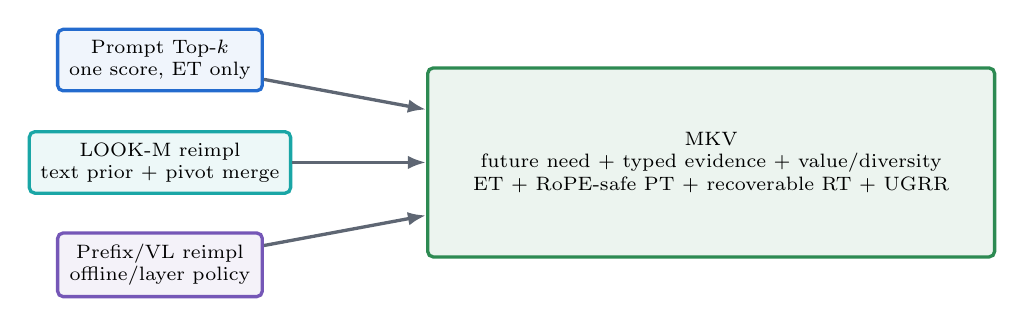
\begin{tikzpicture}[x=1cm,y=1cm]
  \node[mkblue,minimum width=2.6cm] (simple) at (0,1.3) {Prompt Top-$k$\\one score, ET only};
  \node[mkcyan,minimum width=2.6cm] (look) at (0,0) {LOOK-M reimpl\\text prior + pivot merge};
  \node[mkpurple,minimum width=2.6cm] (prefix) at (0,-1.3) {Prefix/VL reimpl\\offline/layer policy};
  \node[mkgreen,minimum width=7.2cm,minimum height=2.4cm] (mkv) at (7.0,0)
    {MKV\\future need + typed evidence + value/diversity\\ET + RoPE-safe PT + recoverable RT + UGRR};
  \draw[mkarrow] (simple)--(mkv); \draw[mkarrow] (look)--(mkv); \draw[mkarrow] (prefix)--(mkv);
\end{tikzpicture}}
\end{center}
\begin{block}{The comparison question}
Does the additional structure preserve more quality or reduce more active bytes after including
its forecast, graph, prototype, and repair overhead?
\end{block}
\end{frame}

% 59 --------------------------------------------------------------------------
\begin{frame}{Fair Comparison Uses Measured Active KV Bytes}
\small
All compared methods must use identical:
\begin{columns}[T,onlytextwidth]
\column{0.48\textwidth}
\begin{itemize}\tightitems
  \item model weights, revision, and precision;
  \item processor, chat template, and tokenization;
  \item prompt text and media preprocessing;
  \item output length and deterministic decoding;
  \item mandatory-token policy where comparable.
\end{itemize}
\column{0.48\textwidth}
\begin{itemize}\tightitems
  \item active KV byte budget;
  \item block size/granularity where applicable;
  \item attention backend;
  \item warmups and timing protocol;
  \item same sample IDs paired across methods.
\end{itemize}
\end{columns}
\begin{alertblock}{Do not compare nominal ratios when bytes differ}
Primary budget = measured active ET/PT KV bytes. RT bytes and metadata are reported separately.
\end{alertblock}
\end{frame}

% 60 --------------------------------------------------------------------------
\begin{frame}{Worked Example, Part 1: Predict, Connect, Score, Choose}
\small
\teachinglabel
\begin{center}
\resizebox{0.92\linewidth}{!}{%
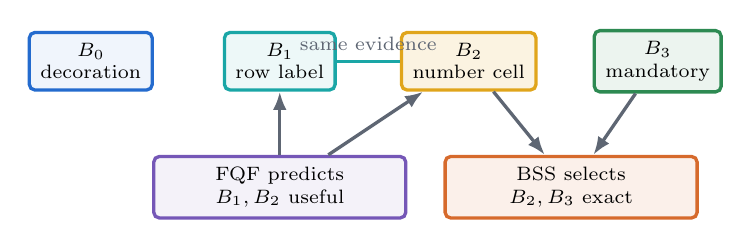
\begin{tikzpicture}[x=1cm,y=1cm]
  \node[mkblue] (b0) at (0,0) {$B_0$\\decoration};
  \node[mkcyan] (b1) at (2.4,0) {$B_1$\\row label};
  \node[mkyellow] (b2) at (4.8,0) {$B_2$\\number cell};
  \node[mkgreen] (b3) at (7.2,0) {$B_3$\\mandatory};
  \node[mkpurple,minimum width=3.2cm] (fq) at (2.4,-1.6) {FQF predicts\\$B_1,B_2$ useful};
  \node[mkorange,minimum width=3.2cm] (sel) at (6.1,-1.6) {BSS selects\\$B_2,B_3$ exact};
  \draw[-,very thick,draw=mkCyan] (b1)--node[above,mklabel] {same evidence}(b2);
  \draw[mkarrow] (fq)--(b1); \draw[mkarrow] (fq)--(b2);
  \draw[mkarrow] (b2)--(sel); \draw[mkarrow] (b3)--(sel);
\end{tikzpicture}}
\end{center}
\begin{block}{Fictional setup}
Four source blocks; active budget holds two exact blocks plus one one-slot PT. $B_3$ is mandatory,
and SCEG connects the row label $B_1$ to number cell $B_2$.
\end{block}
\end{frame}

% 61 --------------------------------------------------------------------------
\begin{frame}{Worked Example, Part 2: Store and Repair}
\footnotesize
\teachinglabel
\begin{center}
\resizebox{0.91\linewidth}{!}{%
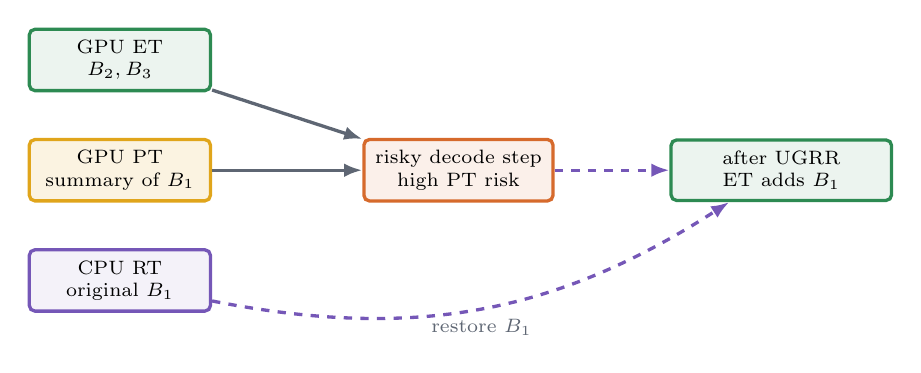
\begin{tikzpicture}[x=1cm,y=1cm]
  \node[mkgreen,minimum width=2.3cm] (et) at (0,1.1) {GPU ET\\$B_2,B_3$};
  \node[mkyellow,minimum width=2.3cm] (pt) at (0,-.3) {GPU PT\\summary of $B_1$};
  \node[mkpurple,minimum width=2.3cm] (rt) at (0,-1.7) {CPU RT\\original $B_1$};
  \node[mkorange,minimum width=2.4cm] (risk) at (4.3,-.3) {risky decode step\\high PT risk};
  \node[mkgreen,minimum width=2.8cm] (after) at (8.4,-.3) {after UGRR\\ET adds $B_1$};
  \draw[mkarrow] (et)--(risk); \draw[mkarrow] (pt)--(risk); \draw[mkdasharrow] (risk)--(after);
  \draw[mkdasharrow] (rt) to[bend right=22] node[below,mklabel] {restore $B_1$} (after);
\end{tikzpicture}}
\end{center}
\begin{alertblock}{Completeness rule}
If an unselected block such as $B_0$ has no safe representation, the planner must find a feasible
exact-only alternative or fail. It cannot silently drop $B_0$ and call the TTC complete.
\end{alertblock}
\end{frame}

% 62 --------------------------------------------------------------------------
\begin{frame}{Label-Free Fidelity Calibration (LFC)}
\small
For calibration sample $x$:
\[
L_x=(1-A_{tok})+\log(1+D_{KL})+E_{attn}+R_{forecast}.
\]
\begin{itemize}\tightitems
  \item $A_{tok}$: token agreement with FullKV.
  \item $D_{KL}$: logit KL divergence.
  \item $E_{attn}$: attention-output error.
  \item $R_{forecast}$: forecast regret.
\end{itemize}
\begin{block}{Selection rule}
Choose the lowest mean + tail fidelity loss under the same measured byte ceiling. Bootstrap
resampling checks profile stability.
\end{block}
\begin{alertblock}{Leakage rule}
Calibration and evaluation IDs are disjoint; no benchmark answer labels select the profile.
\end{alertblock}
\end{frame}

% 63 --------------------------------------------------------------------------
\begin{frame}{Six Quality Safeguards around the Core Design}
\scriptsize
\begin{enumerate}\tightitems
  \item \textbf{PAR}: preserve direct prompt evidence.
  \item \textbf{LFC}: choose a stable label-free fidelity profile.
  \item \textbf{PHR}: route stable/shifted forecast heads and PT-sensitive heads differently.
  \item \textbf{EPR}: preserve fine chart/document evidence.
  \item \textbf{PKT}: merge post-RoPE keys only in phase-neutral space.
  \item \textbf{DAR}: trigger restoration only under calibrated risk/decision conditions.
\end{enumerate}
\begin{alertblock}{Evidence requirement}
These are implemented safeguards, not proof of general superiority. Held-out, clean-worktree,
byte-matched experiments must show whether they improve the quality--memory frontier.
\end{alertblock}
\end{frame}

\section{Implementation, Measurement, and Support}

% 64 --------------------------------------------------------------------------
\begin{frame}[fragile]{Runtime Pseudocode}
\begin{lstlisting}[style=mosaickv,language={}]
prepared = adapter.prepare_inputs(messages, media)
prefill = adapter.prefill(prepared, capture_queries=True,
                         capture_attentions=True)

full = blockize(adapter.extract_past_key_values(prefill),
                logical_positions, modality_spans)
forecast, draft = forecast_with_rollout(prefill)
attention = pool_rope_aware_prompt_and_draft_attention(prefill, draft)

graph = build_evidence_graph(full)
utility = compute_block_utilities(graph, attention)
selected = lazy_greedy_select(utility, graph, active_byte_budget)
tiers = construct_three_tier_cache(full, selected, graph,
                                   adapter.prototype_key_transform)

state = pack_and_inject(tiers, keep_logical_positions=True)
for step in decode_steps:
    provisional = adapter.decode_one_token(token, state)
    repair = maybe_restore_residuals(provisional, state)
    token, state = accept_or_redecode_once(provisional, repair)
\end{lstlisting}
\end{frame}

% 65 --------------------------------------------------------------------------
\begin{frame}{Dense Physical Cache Budget (DPCB)}
\small
\begin{columns}[T,onlytextwidth]
\column{0.50\textwidth}
\begin{block}{Logical selection}
BSS may choose different position counts for different layer/head pairs.
\end{block}
\begin{block}{Physical allocation}
A dense HF tensor may allocate using a common maximum packed length. Logical cost can therefore
differ from real storage.
\end{block}
\column{0.46\textwidth}
\begin{exampleblock}{DPCB job}
\begin{itemize}\tightitems
  \item quantize the request to representable whole-block capacity;
  \item set per-layer/head position limits;
  \item verify packed tensor bytes;
  \item report requested and realized RR.
\end{itemize}
\end{exampleblock}
\end{columns}
\begin{alertblock}{\whylabel}
Counting selected blocks while allocating a larger dense cache would overstate memory savings.
\end{alertblock}
\end{frame}

% 66 --------------------------------------------------------------------------
\begin{frame}{Packing and Decode Masks}
\small
\begin{itemize}\tightitems
  \item Sort ET entries by original logical position inside every layer/head.
  \item Place PT entries at their selected-anchor logical positions.
  \item Use an all-valid fast path when packed capacities align.
  \item Otherwise build checked per-layer/head validity masks for eager attention.
  \item Append generated physical slots while advancing original logical positions.
\end{itemize}
\begin{alertblock}{NaN/Inf safety}
The runtime checks packed K/V, attention masks, prefill logits, and decode logits for not-a-number
(NaN) and infinity (Inf). A compressed state without a valid logical-position mask is rejected.
\end{alertblock}
\end{frame}

% 67 --------------------------------------------------------------------------
\begin{frame}{Measurement Boundaries}
\scriptsize
\begin{center}
\resizebox{0.97\linewidth}{!}{%
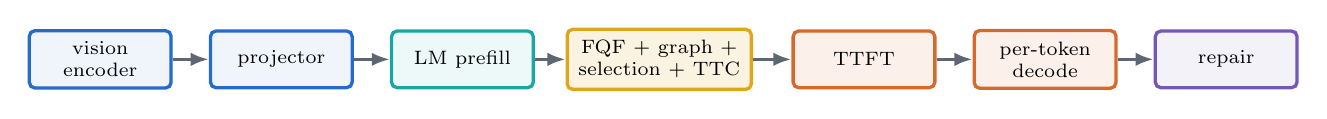
\begin{tikzpicture}[x=1cm,y=1cm]
  \node[mkblue,minimum width=1.8cm] (vision) at (0,0) {vision\\encoder};
  \node[mkblue,minimum width=1.8cm] (proj) at (2.3,0) {projector};
  \node[mkcyan,minimum width=1.8cm] (prefill) at (4.6,0) {LM prefill};
  \node[mkyellow,minimum width=2.0cm] (comp) at (7.1,0) {FQF + graph +\\selection + TTC};
  \node[mkorange,minimum width=1.8cm] (ttft) at (9.7,0) {TTFT};
  \node[mkorange,minimum width=1.8cm] (decode) at (12.0,0) {per-token\\decode};
  \node[mkpurple,minimum width=1.8cm] (repair) at (14.3,0) {repair};
  \draw[mkarrow] (vision)--(proj); \draw[mkarrow] (proj)--(prefill);
  \draw[mkarrow] (prefill)--(comp); \draw[mkarrow] (comp)--(ttft);
  \draw[mkarrow] (ttft)--(decode); \draw[mkarrow] (decode)--(repair);
\end{tikzpicture}}
\end{center}
\begin{block}{GPU timing rule}
Use \code{torch.cuda.Event} and \code{torch.cuda.synchronize} at every timing boundary. Retain every
trial and derive median, p5, p95, mean, standard deviation, and bootstrap confidence interval.
\end{block}
\begin{alertblock}{\whylabel}
GPU work is asynchronous. A host timer can stop before the GPU finishes and report false speedups.
\end{alertblock}
\end{frame}

% 68 --------------------------------------------------------------------------
\begin{frame}{Memory Accounting}
\small
Record four different memory views:
\begin{enumerate}\tightitems
  \item active ET/PT K/V bytes from tensor storage;
  \item CPU RT bytes from the actual residual encoding;
  \item peak GPU memory allocated;
  \item peak GPU memory reserved.
\end{enumerate}
\begin{block}{Exact active-byte rule}
\[
\text{tensor bytes}=\operatorname{numel}(T)\times\operatorname{element\_size}(T),
\]
with view/underlying storage handled consistently across methods.
\end{block}
\begin{alertblock}{Repair accounting}
Record restored bytes, transfer time, re-decode time, and active cost before/after every event.
\end{alertblock}
\end{frame}

% 69 --------------------------------------------------------------------------
\begin{frame}{Every Run Has an Immutable Manifest}
\scriptsize
Every experimental row resolves to:
\begin{columns}[T,onlytextwidth]
\column{0.48\textwidth}
\begin{itemize}\tightitems
  \item Git and config SHA;
  \item dirty-worktree and patch identity;
  \item model ID and immutable revision;
  \item dataset ID and revision;
  \item seed and measurement type;
  \item prompt/media/tokenization identity.
\end{itemize}
\column{0.48\textwidth}
\begin{itemize}\tightitems
  \item CUDA and driver versions;
  \item PyTorch, Transformers, vLLM, SGLang;
  \item GPU type/count, power, and clocks;
  \item background GPU processes;
  \item backend, attention implementation, precision;
  \item generation/output policy.
\end{itemize}
\end{columns}
\begin{alertblock}{Canonical-run rule}
A dirty-worktree run is exploratory even when its patch is preserved. Missing provenance never
becomes an empty field; use an explicit value such as \code{not_used}.
\end{alertblock}
\end{frame}

% 70 --------------------------------------------------------------------------
\begin{frame}{The Debug Trace Explains Every Decision}
\small
One trace per attempted sample includes:
\begin{itemize}\tightitems
  \item FQF statistics and attention provenance;
  \item SCEG nodes and typed edges;
  \item every VBU signal and BSS marginal gain/reason;
  \item ET/PT/RT membership and PKT provenance;
  \item packed slots and logical positions;
  \item UGRR signals, restored blocks, and re-decode outcome;
  \item generated token IDs, bytes, and timing breakdown.
\end{itemize}
\begin{alertblock}{Failure visibility}
A failed sample writes an error result and failed trace. It never silently disappears from the
sample ledger.
\end{alertblock}
\end{frame}

% 71 --------------------------------------------------------------------------
\begin{frame}{Testing Progression}
\small
\begin{center}
\resizebox{0.90\linewidth}{!}{%
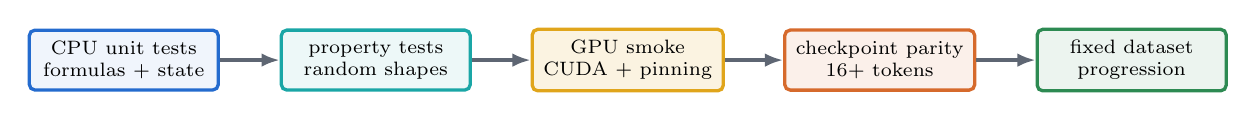
\begin{tikzpicture}[x=1cm,y=1cm]
  \node[mkblue,minimum width=2.4cm] (cpu) at (0,0) {CPU unit tests\\formulas + state};
  \node[mkcyan,minimum width=2.4cm] (pbt) at (3.2,0) {property tests\\random shapes};
  \node[mkyellow,minimum width=2.4cm] (gpu) at (6.4,0) {GPU smoke\\CUDA + pinning};
  \node[mkorange,minimum width=2.4cm] (model) at (9.6,0) {checkpoint parity\\16+ tokens};
  \node[mkgreen,minimum width=2.4cm] (data) at (12.8,0) {fixed dataset\\progression};
  \draw[mkarrow] (cpu)--(pbt); \draw[mkarrow] (pbt)--(gpu);
  \draw[mkarrow] (gpu)--(model); \draw[mkarrow] (model)--(data);
\end{tikzpicture}}
\end{center}
\begin{block}{Evidence levels are different}
Synthetic tests prove formulas and invariants. Real checkpoints prove model compatibility. Clean,
sufficiently sized datasets are still required for scientific quality claims.
\end{block}
\end{frame}

% 72 --------------------------------------------------------------------------
\begin{frame}{Key Correctness Gates}
\scriptsize
\begin{tabularx}{\textwidth}{>{\bfseries}p{0.22\textwidth}X}
\toprule
Gate & Required behavior \\
\midrule
FullKV parity & Explicit loop matches ordinary greedy generation. \\
Extract/reinject & Cache round trip preserves greedy tokens and bounded logits. \\
RR = 1.0 & Every source block exact; no PT/RT/UGRR transformation. \\
DR isolation & Original prefill K/V and state unchanged after forecast. \\
BSS budget & Deterministic, mandatory retained, active bytes never exceed target. \\
PT safety & Same layer/head and compatible RoPE phases only. \\
UGRR state & Policy none never triggers; one re-decode maximum; budget remains valid. \\
Oracle isolation & True future Q/repair decisions unavailable to online code. \\
\bottomrule
\end{tabularx}
\end{frame}

% 73 --------------------------------------------------------------------------
\begin{frame}{Current HF Model Support Boundary}
\scriptsize
\begin{tabularx}{\textwidth}{>{\bfseries}p{0.22\textwidth}c c c X}
\toprule
Family & Exact HF & PT & UGRR & Boundary \\
\midrule
Qwen2.5-VL & supported & conditional & conditional & Audited M-RoPE PKT; eager PT/UGRR path. \\
LLaVA-1.5 & supported & conditional & conditional & Audited standard Llama RoPE PKT. \\
LLaVA-OneVision & supported & conditional & conditional & Audited standard Qwen2 RoPE PKT. \\
InternVL2.5 & conditional & unsupported & unsupported & Optional remote-code exact-only adapter. \\
\bottomrule
\end{tabularx}
\begin{alertblock}{Meaning of conditional}
The runtime checks Transformers version, attention path, padding/position layout, cache key state,
and PKT provenance. Any mismatch fails closed.
\end{alertblock}
\end{frame}

% 74 --------------------------------------------------------------------------
\begin{frame}{Attention Backend Boundary}
\small
\begin{itemize}\tightitems
  \item FullKV can use eager, Scaled Dot-Product Attention (SDPA), or FlashAttention-2 (FA2) where
        the adapter and installed environment declare support.
  \item SCEG/VBU selection requiring explicit attention begins with eager prefill evidence.
  \item PT and live UGRR currently require the owned eager path.
  \item An all-valid exact cache may switch to an audited faster decode attention implementation.
  \item Padded per-head PT/UGRR fused paths remain unsupported until parity is proven.
\end{itemize}
\begin{alertblock}{No hidden switching}
Prefill and decode attention implementations are both recorded in configuration, manifest, and
trace.
\end{alertblock}
\end{frame}

% 75 --------------------------------------------------------------------------
\begin{frame}{vLLM and SGLang Boundary}
\small
\begin{columns}[T,onlytextwidth]
\column{0.48\textwidth}
\begin{block}{What exists}
\begin{itemize}\tightitems
  \item FullKV measurement wrappers;
  \item version-pinned whole-block transport tests;
  \item logical-position and request-isolation checks.
\end{itemize}
\end{block}
\column{0.48\textwidth}
\begin{alertblock}{What is not a paper MKV row}
\begin{itemize}\tightitems
  \item fallback-selector transport test;
  \item unverified common-selector bridge;
  \item serving PT injection;
  \item serving RT/UGRR.
\end{itemize}
\end{alertblock}
\end{columns}
\begin{block}{Why native integration is hard}
The engine jointly owns physical K/V, block tables, scheduler state, prefix/Radix metadata, and
logical positions. Updating only tensors would leave inconsistent state.
\end{block}
\end{frame}

% 76 --------------------------------------------------------------------------
\begin{frame}{Known Limitations and Risks}
\scriptsize
\begin{enumerate}\tightitems
  \item FQF, SCEG, BSS, PKT, packing, and UGRR add compression latency.
  \item A short DR may miss evidence needed much later.
  \item SCEG quality depends on real metadata availability.
  \item Even RoPE-safe PT can blur distinct content vectors.
  \item UGRR can trigger on an uncertain but correct token; DAR may disable itself.
  \item Dense HF layouts can reduce physical savings relative to logical selection.
  \item RT saves active GPU memory but uses CPU memory and transfer/conversion work.
  \item Serving-engine full TTC/UGRR transactions remain unsupported.
  \item Small or dirty-worktree runs do not prove general superiority.
\end{enumerate}
\end{frame}

% 77 --------------------------------------------------------------------------
\begin{frame}{How to Read a Future MKV Result}
\scriptsize
Ask in this order:
\begin{enumerate}\tightitems
  \item Did RR $=1.0$ pass FullKV token/logit parity?
  \item Were model, media, prompt, processor, output, and decoding identical?
  \item Are budgets measured active KV bytes?
  \item Did real PT/RT/UGRR run, or was it an exact-only fallback?
  \item Are compression and repair included in E2E latency?
  \item Are RT bytes separate from active bytes?
  \item Are official per-task scores kept separate before any normalized macro average?
  \item Are failed samples, seeds, and trials preserved?
  \item Does the manifest point to a clean Git SHA and immutable revisions?
  \item Do held-out paired confidence intervals support the conclusion?
\end{enumerate}
\end{frame}

% 78 --------------------------------------------------------------------------
\begin{frame}{Final Takeaways}
\small
\begin{enumerate}\tightitems
  \item MKV is not one top-$k$ score; it is a six-component prediction, evidence, selection,
        representation, and correction pipeline.
  \item Logical positions, exact bytes, and RoPE phase are correctness requirements, not optional
        implementation details.
  \item ET is universal; PT and UGRR are enabled only through audited model-specific paths.
  \item RT makes selected approximation errors recoverable, but memory and latency remain visible.
  \item A safe fallback is better than an invalid prototype or simulated native backend row.
  \item Final superiority must be demonstrated with clean, held-out, byte-matched experiments.
\end{enumerate}
\begin{exampleblock}{One last notebook analogy}
Predict the next questions, connect notes about the same fact, pack a diverse backpack, summarize
only compatible pages, and reopen the drawer only when the answer decision looks fragile.
\end{exampleblock}
\end{frame}

\appendix
\section{Appendix}

% 79 --------------------------------------------------------------------------
\begin{frame}{Appendix: Source Map I}
\scriptsize
Paths are relative to \code{mosaickv/}.
\begin{tabularx}{\textwidth}{>{\bfseries}p{0.24\textwidth}p{0.37\textwidth}X}
\toprule
Concept & Source & Main object \\
\midrule
Configuration & \code{src/mosaickv/config.py} & \code{RunConfig} and strict component configs \\
Adapter contract & \code{src/mosaickv/adapters/huggingface/} & \code{AdapterCapabilities}, \code{DecodeState} \\
FullKV & \code{src/mosaickv/fullkv.py} & synchronized reference runner \\
Cache state & \code{src/mosaickv/cache_state.py} & KVBD, LPM, \code{FullKVState}, \code{MosaicKVState} \\
FQF & \code{src/mosaickv/forecasting/} & \code{QueryForecast}, isolated rollout \\
SCEG & \code{src/mosaickv/graph/} & \code{SparseEvidenceGraph}, pooling, diagnostics \\
VBU/BSS & \code{src/mosaickv/selection/} & utility, objective, lazy/exhaustive selectors \\
\bottomrule
\end{tabularx}
\end{frame}

% 80 --------------------------------------------------------------------------
\begin{frame}{Appendix: Source Map II}
\scriptsize
\begin{tabularx}{\textwidth}{>{\bfseries}p{0.24\textwidth}p{0.37\textwidth}X}
\toprule
Concept & Source & Main object \\
\midrule
LFC/PHR & \code{src/mosaickv/selection/calibration.py} & frozen fidelity profile and head routing \\
TTC/PT & \code{src/mosaickv/prototypes/} & TTC constructor and PT records \\
PKT & \code{src/mosaickv/prototypes/rope.py} & \code{RotaryPrototypeKeyTransform} \\
RT & \code{src/mosaickv/residual/} & pinned and quantized CPU storage \\
UGRR/DAR & \code{src/mosaickv/repair/} & repair state, controller, calibration, oracle isolation \\
HF runtime & \code{src/mosaickv/backends/hf_runtime.py} & compression plan, packing, explicit decode \\
Measurement & \code{src/mosaickv/measurements/} & CUDA timing, bytes, telemetry, statistics \\
Evaluation & \code{src/mosaickv/evaluation/} & task registry, JSONL/Parquet, resume and merge \\
\bottomrule
\end{tabularx}
\end{frame}

% 81 --------------------------------------------------------------------------
\begin{frame}[fragile]{Appendix: YAML Configuration Shape}
\scriptsize
\begin{lstlisting}[style=mosaickv,language={},basicstyle=\tiny\ttfamily]
method: mosaickv_full
cache:
  block_size: 16
  retention_ratio: 0.40
  budget_unit: bytes
forecasting:
  mode: hybrid
  prompt_window: 16
  draft_steps: 4
graph:
  max_neighbors: 8
selection:
  algorithm: lazy_greedy
  prompt_anchor_fraction: 0.05
  evidence_preservation_fraction: 0.05
prototypes:
  enabled: true
  group_size: 4
residual:
  enabled: true
  storage_dtype: lossless
repair:
  policy: decision_aware
  max_blocks_per_step: 1
\end{lstlisting}
\teachinglabel: this is a schema example, not a recommended paper configuration.
\end{frame}

% 82 --------------------------------------------------------------------------
\begin{frame}{Appendix: Checklist for a New Model Adapter}
\scriptsize
\begin{enumerate}\tightitems
  \item Pin model/processor revisions and inspect exact public source.
  \item Record media, attention, cache-class, layout, and sequence-axis capabilities.
  \item Implement the checkpoint chat template and media processor.
  \item Implement one prefill and explicit deterministic one-token decode.
  \item Capture Q at \code{q_proj} without changing weights.
  \item Determine cached-K RoPE state from source.
  \item Pass ordinary generation, extraction/reinjection, and RR = 1.0 parity.
  \item Enable PT only after an audited PKT and real TTC safety gate.
  \item Enable UGRR only after pinned RT, partial refresh, one-redecode, and budget tests.
  \item Add the exact boundary to model/backend capability matrices.
\end{enumerate}
\end{frame}

% 83 --------------------------------------------------------------------------
\begin{frame}{Appendix: Detailed Design References}
\scriptsize
\begin{columns}[T,onlytextwidth]
\column{0.49\textwidth}
\begin{itemize}\tightitems
  \item \code{docs/mosaickv_design_and_implementation.tex}
  \item \code{docs/cache_state.md}
  \item \code{docs/future_query_forecasting.md}
  \item \code{docs/evidence_graph.md}
  \item \code{docs/block_utility_and_selection.md}
  \item \code{docs/three_tier_cache.md}
\end{itemize}
\column{0.47\textwidth}
\begin{itemize}\tightitems
  \item \code{docs/decode_time_repair.md}
  \item \code{docs/huggingface_adapters.md}
  \item \code{docs/huggingface_runtime.md}
  \item \code{docs/model_capability_matrix.md}
  \item \code{docs/backend_capability_matrix.md}
  \item \code{SCIENTIFIC_INTEGRITY.md}
  \item \code{REPRODUCIBILITY.md}
\end{itemize}
\end{columns}
\end{frame}

\end{document}
